\documentclass[12pt]{beamer}

\usepackage{beamerthemesplit}


\usepackage{beamerthemesplit}

\usepackage{beamerStatisticsTAMU} 

\logo{\includegraphics[height=1.5cm]{STAT_Horz-Aggie-Maroon.pdf}\vspace{220pt}}


\usepackage{amsmath}
\usepackage{amssymb}
\usepackage{verbatim}
\usepackage{bibentry}
%\usepackage{biblatex}
%\usepackage{natbib}
\newcommand{\argmin}[1]{\underset{#1}{\operatorname{argmin}}\text{ }}
\newcommand{\argmax}[1]{\underset{#1}{\operatorname{argmax}}\text{ }}
\usepackage{bbm}
\usepackage{bm}
\usepackage[absolute,overlay]{textpos}

\newcommand{\Var}{\text{Var }}
\newcommand{\Cov}{\text{Cov }}
\newcommand{\E}{\mathbb{E}}
\newcommand{\ind}{\mathbbm{1}}
\newcommand{\V}[1]{{\bm{\mathbf{\MakeLowercase{#1}}}}} % vector
\newcommand{\M}[1]{{\bm{\mathbf{\MakeUppercase{#1}}}}} % matrix
\newcommand{\todo}[1]{{\color{red}TODO: #1}}
\newcommand{\tikzmark}[1]{\tikz[overlay,remember picture] \node (#1) {};}
\newcommand{\w}{1in}
\newcommand{\h}{1in}

\usepackage{graphicx}
\newcommand{\indep}{\rotatebox[origin=c]{90}{$\models$}}

\newtheorem{assumptions}{Assumptions}

\setbeamertemplate{headline}[default]
\setbeamertemplate{footline}[page number]
\setbeamertemplate{navigation symbols}{}
\setbeamertemplate{bibliography item}[text]

\title{Statistical Tools for Time Domain Astronomy}
\author{James Long}
\institute{Texas A\&M University}
\date{\today}
\begin{document}

\frame{\titlepage}

\frame{\tableofcontents}

\AtBeginSection[]
{
  \begin{frame}<beamer>
    \frametitle{Outline}
    \tableofcontents[currentsection,currentsubsection]
  \end{frame}
}


%%%%%%%%
%%%%%%%% TODO: redo first section with more emphasis on multiband, lomb scargle
%%%%%%%%


\begin{frame}{Texas A\&M Collaboration}

%% astronomers
%%   \begin{textblock*}{12cm}(0cm,1cm) % {block width} (coords)
%% \begin{center}
%% \textbf{Astronomy}
%% \end{center}
%% \end{textblock*}
%%   \begin{textblock*}{3cm}(3.5cm,2cm) % {block width} (coords)
%% 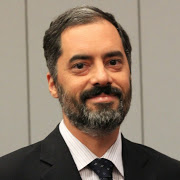
\includegraphics[width=\w,height=\h]{figs/Macri.jpg}\\
%% Lucas Macri
%% \end{textblock*}
%%   \begin{textblock*}{3cm}(7cm,2cm) % {block width} (coords)
%% 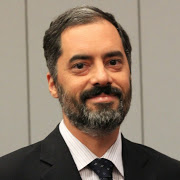
\includegraphics[width=\w,height=\h]{figs/Macri.jpg}\\
%% Wenlong Yuan
%% \end{textblock*}


%% statisticians
  \begin{textblock*}{3cm}(1.5cm,3.1cm) % {block width} (coords)
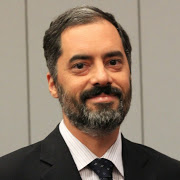
\includegraphics[width=\w,height=\h]{figs/Macri.jpg}\\
Lucas Macri
\end{textblock*}


  \begin{textblock*}{3cm}(5cm,3.1cm) % {block width} (coords)
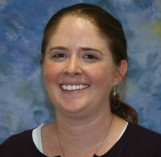
\includegraphics[width=\w,height=\h]{figs/marshall.jpg}\\
Jennifer Marshall
\end{textblock*}

  \begin{textblock*}{3cm}(8.5cm,3.1cm) % {block width} (coords)
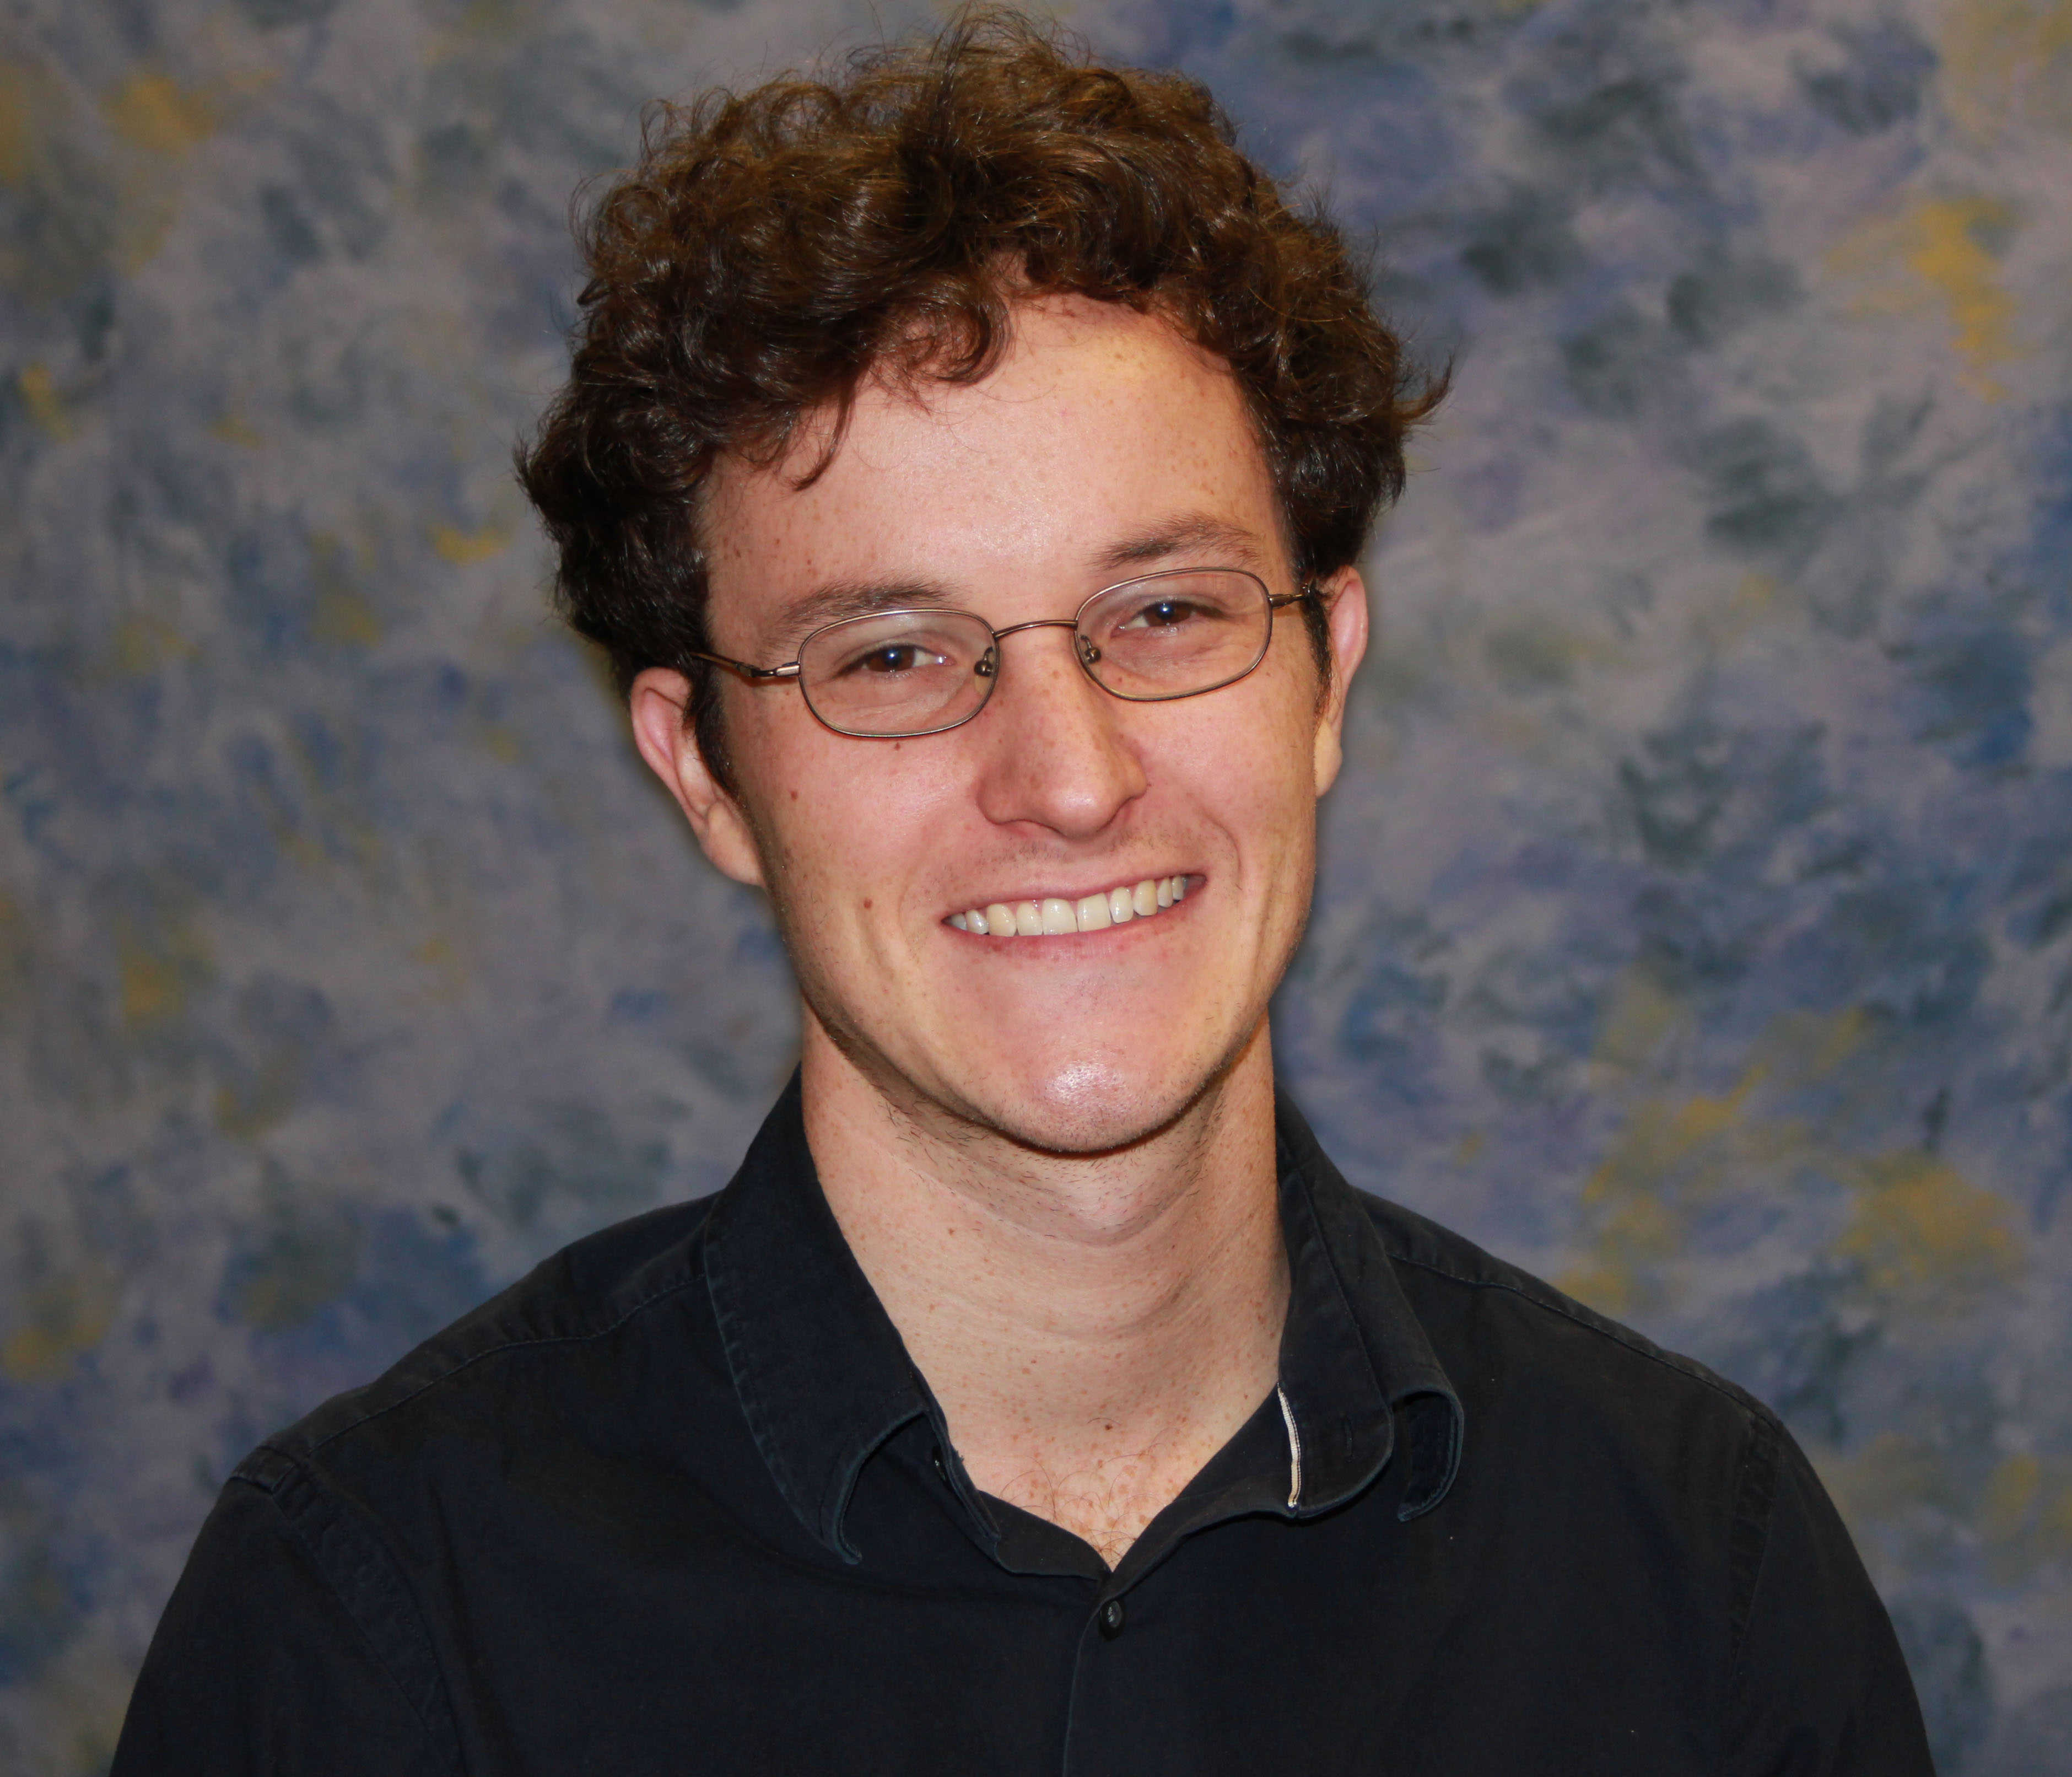
\includegraphics[width=\w,height=\h]{figs/long.jpg}\\
James Long
\end{textblock*}


\end{frame}


\begin{frame}{Why Important?}

  Abstract: Ongoing and upcoming time domain surveys will produce
unprecedented amounts of data. Turning these data into scientific
knowledge requires application and development of sophisticated
statistical methodology. I will discuss some new statistical tools for
analyzing time domain data, including period estimators for sparsely
sampled periodic variable stars and machine learning algorithms for
source classification. I will highlight the concept of the
bias--variance tradeoff in both of these problems and discuss methods
such as cross validation for optimizing this tradeoff. I will conclude
with an application of these methods to finding structure in the Milky
Way Halo using Dark Energy Survey data.



  \end{frame}



\section{Motivating Problem: Mapping the Galactic Halo}

\begin{frame}{Periodic Variable Stars}
\textbf{Periodic variables:} Stars that repeat brightness variation over a fixed period.
\begin{center}
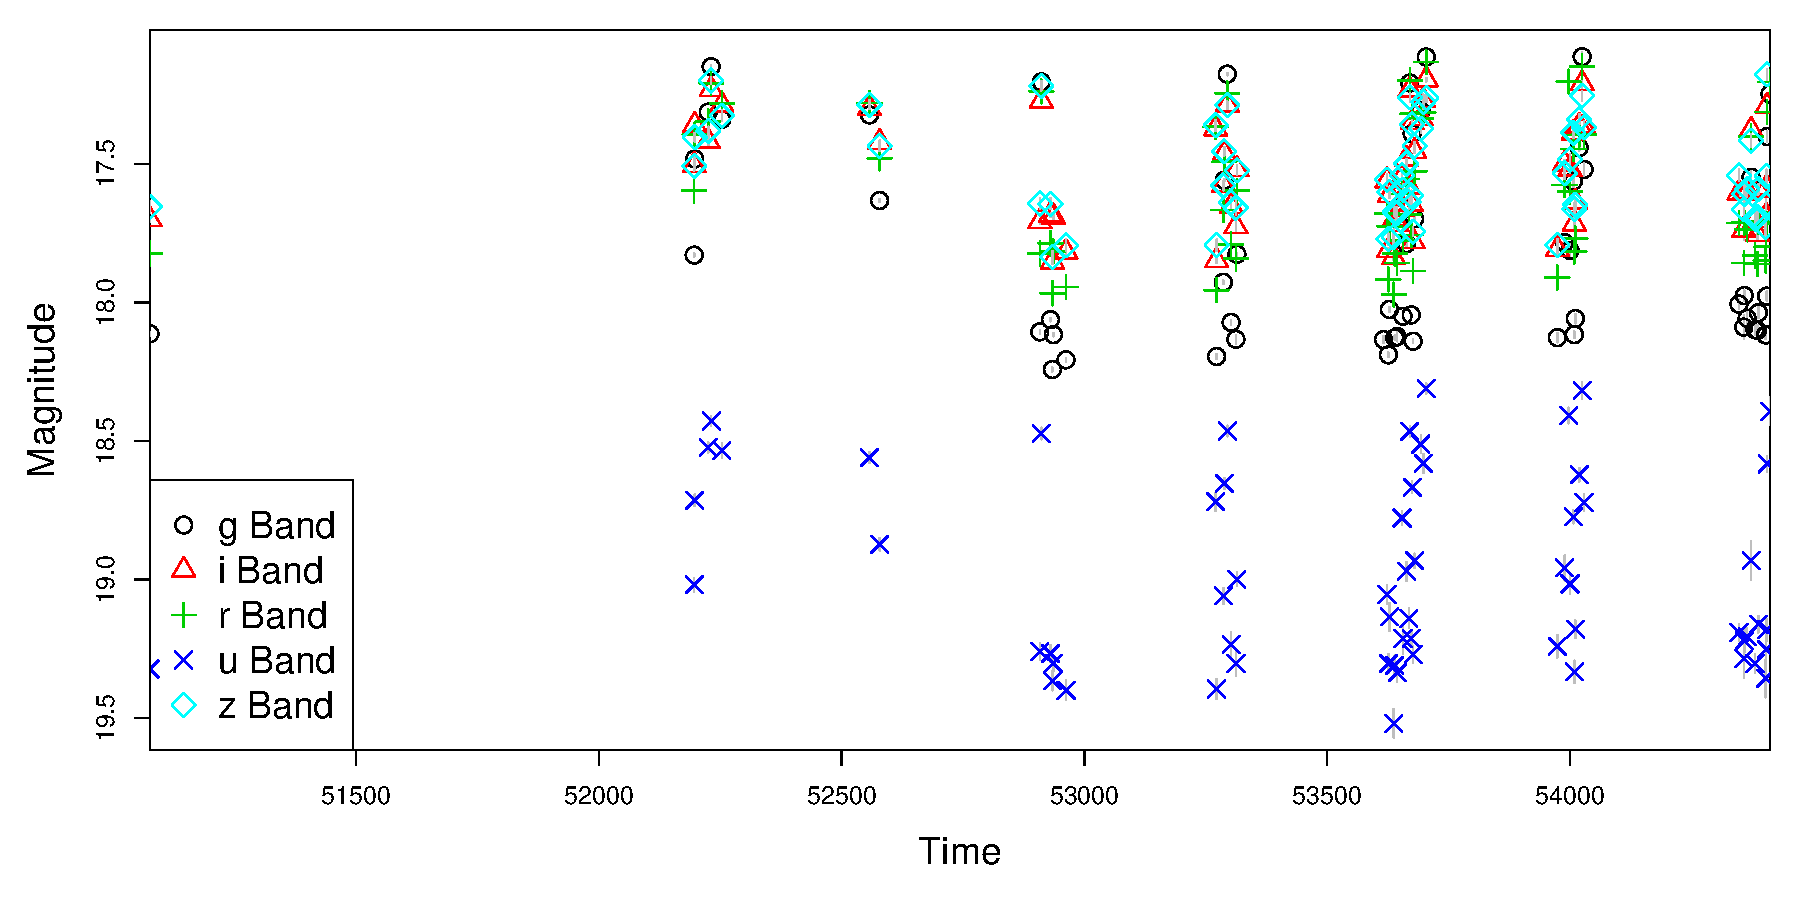
\includegraphics[scale=.3]{figs/unfolded_13350.pdf}
\end{center}
\begin{itemize}
\item Star observed $\approx 250$ times in $5$ bands, $u,g,r,i,z$.
\item Data for star is $D=\{t_{jb},m_{jb},\sigma_{jb}\}_{j=1}^{n_b}$ for $b=1,\ldots,B$.
\item Observe brightness $m_{jb}$ at time $t_{jb}$ with uncertainty $\sigma_{jb}$ in band $b$.
\end{itemize}
\end{frame}


\begin{frame}{Folded Light Curve of Periodic Variable}
\textbf{Folded light curve:} Brightness versus time modulo period.
\begin{center}
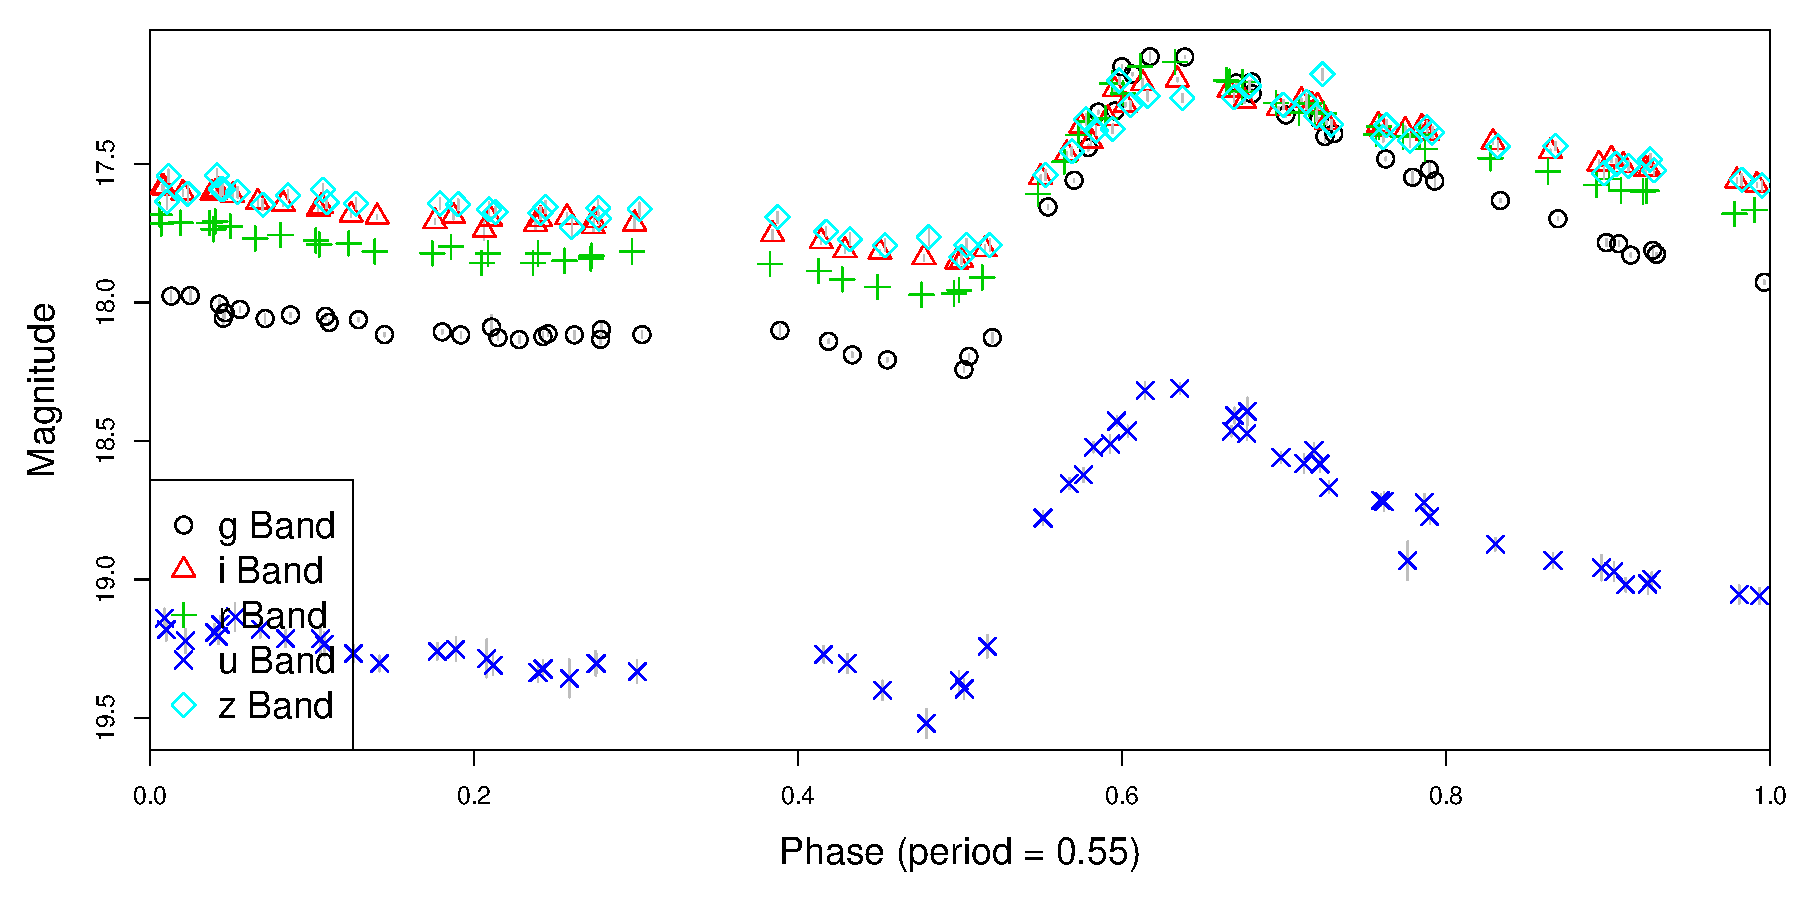
\includegraphics[scale=.3]{figs/folded_13350.pdf}
\end{center}
\end{frame}


\begin{frame}{SDSS--III Stripe 82 \cite{ivezic2007sloan}}
\begin{itemize}
\item Collected $\approx 60,000$ variables in Stripe 82 Region
\item Variables belong to different \textbf{classes}
\item Some periodic, some not
\end{itemize}


\underline{Two Examples}

\vspace{-.2in}

\begin{center}
Eclipsing Binary\\
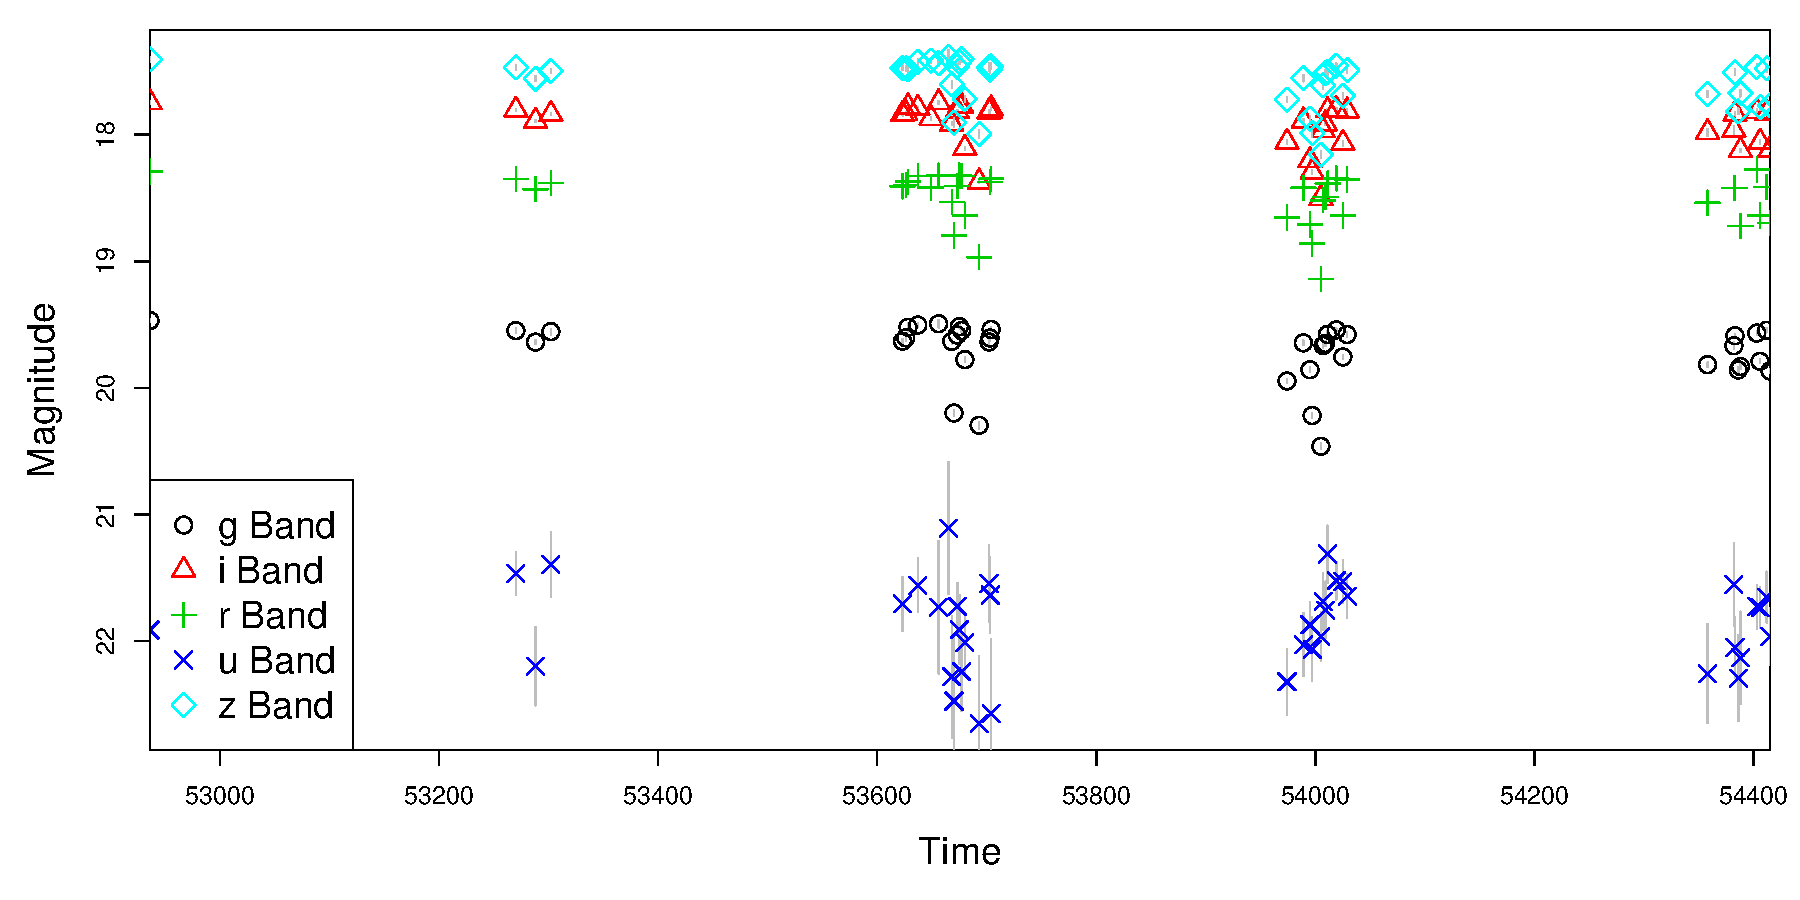
\includegraphics[scale=.15]{figs/unfolded_4183016.pdf}
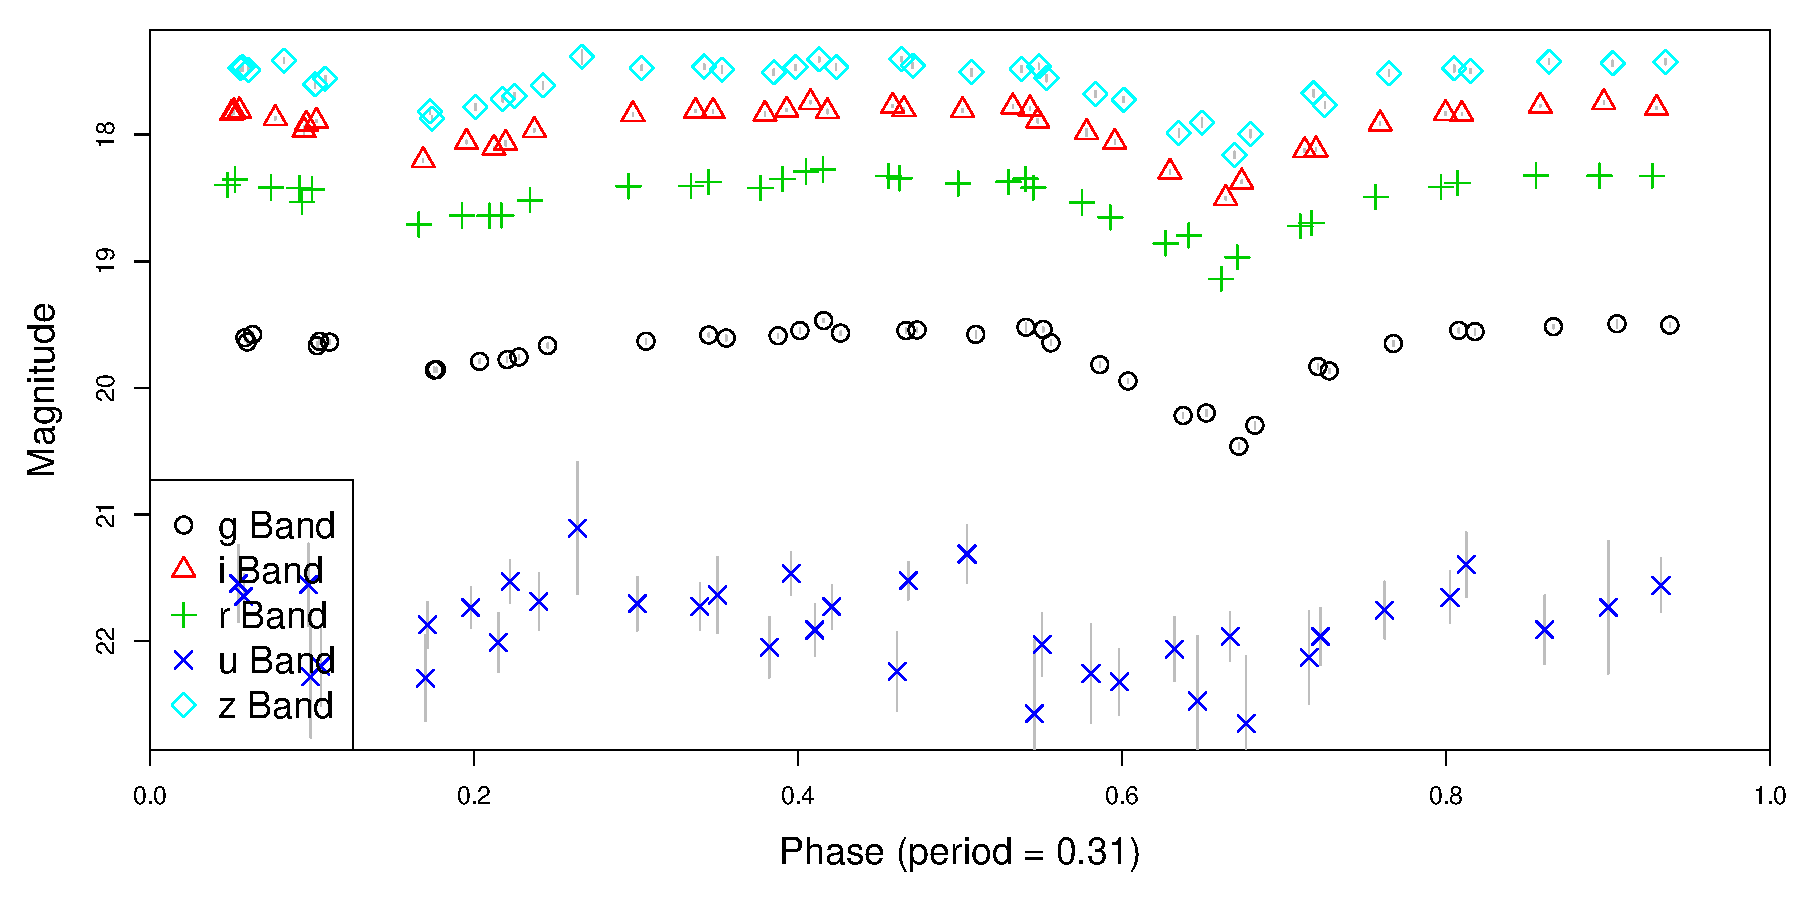
\includegraphics[scale=.15]{figs/folded_4183016.pdf}
\end{center}

\vspace{-.2in}

%% \begin{center}
%% RR Lyrae\\
%% 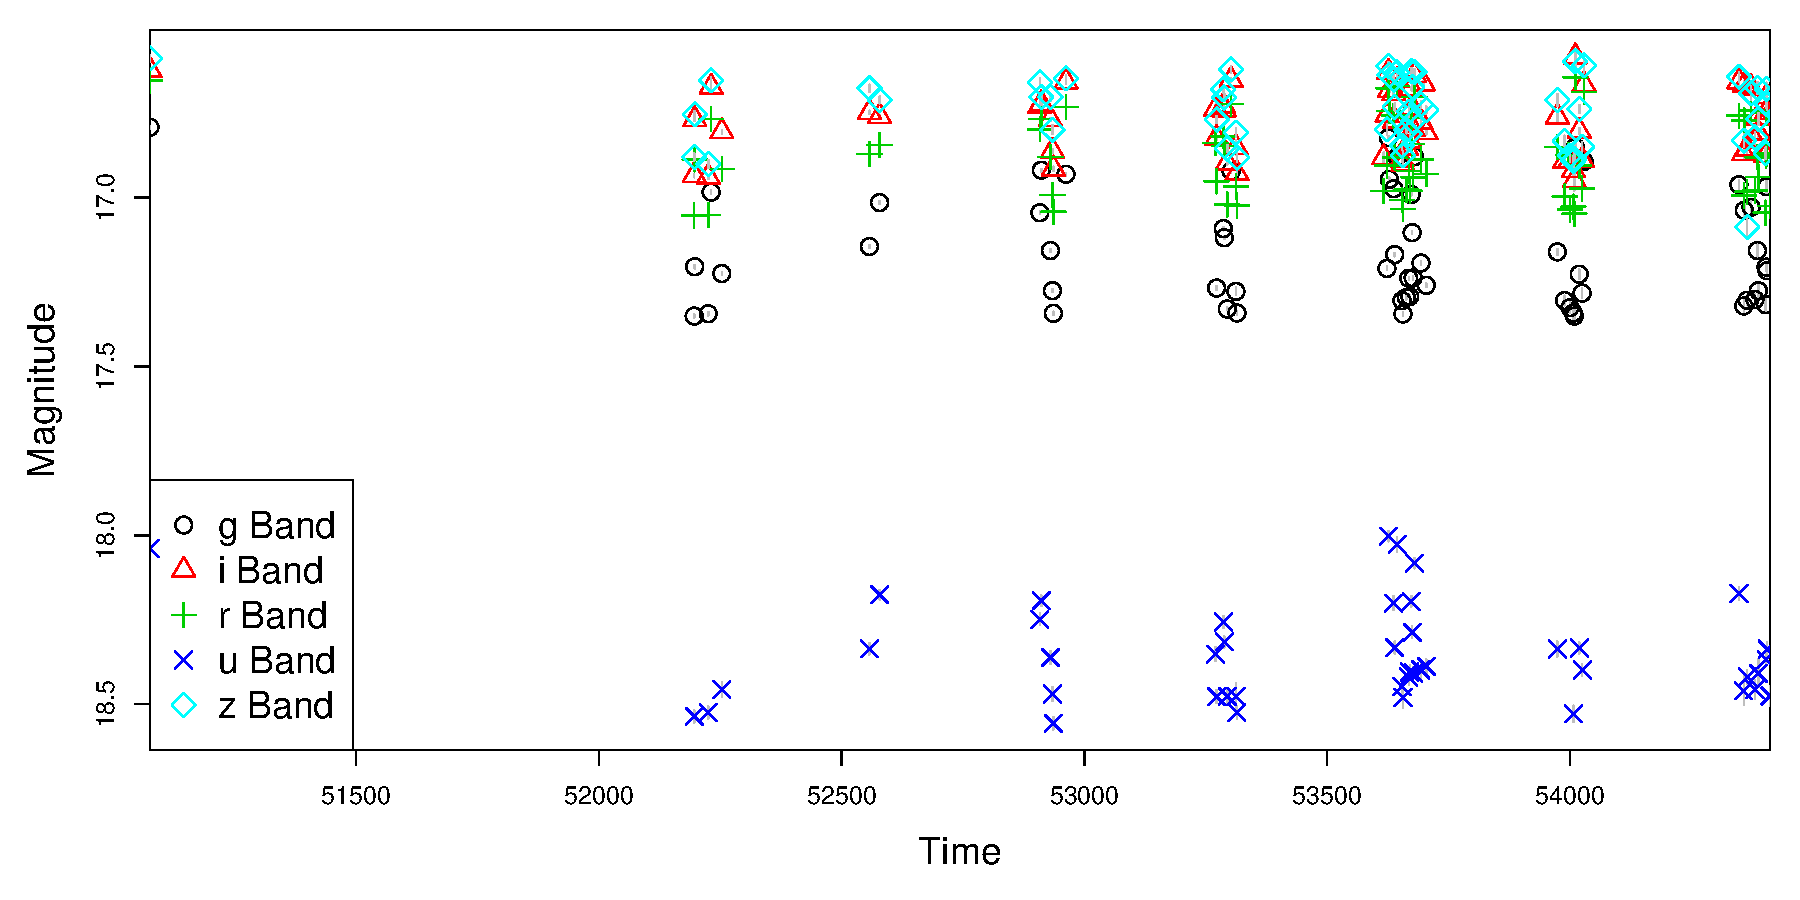
\includegraphics[scale=.15]{figs/unfolded_4099.pdf}
%% 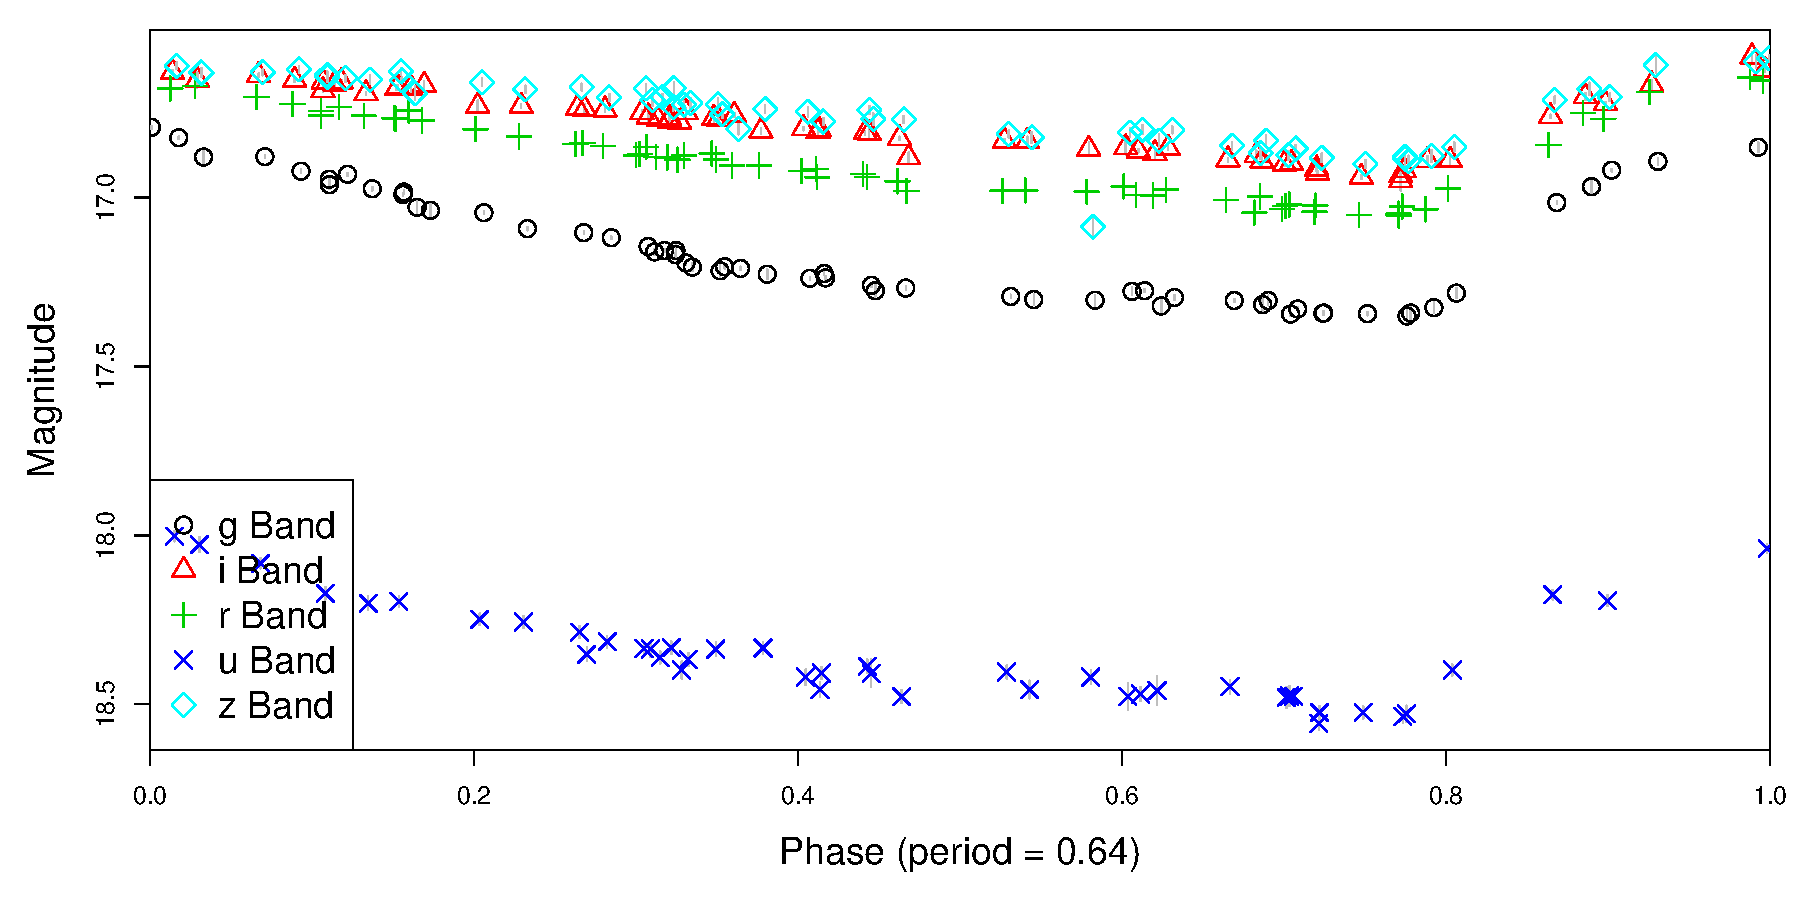
\includegraphics[scale=.15]{figs/folded_4099.pdf}
%% \end{center}


\begin{center}
Quasar\\
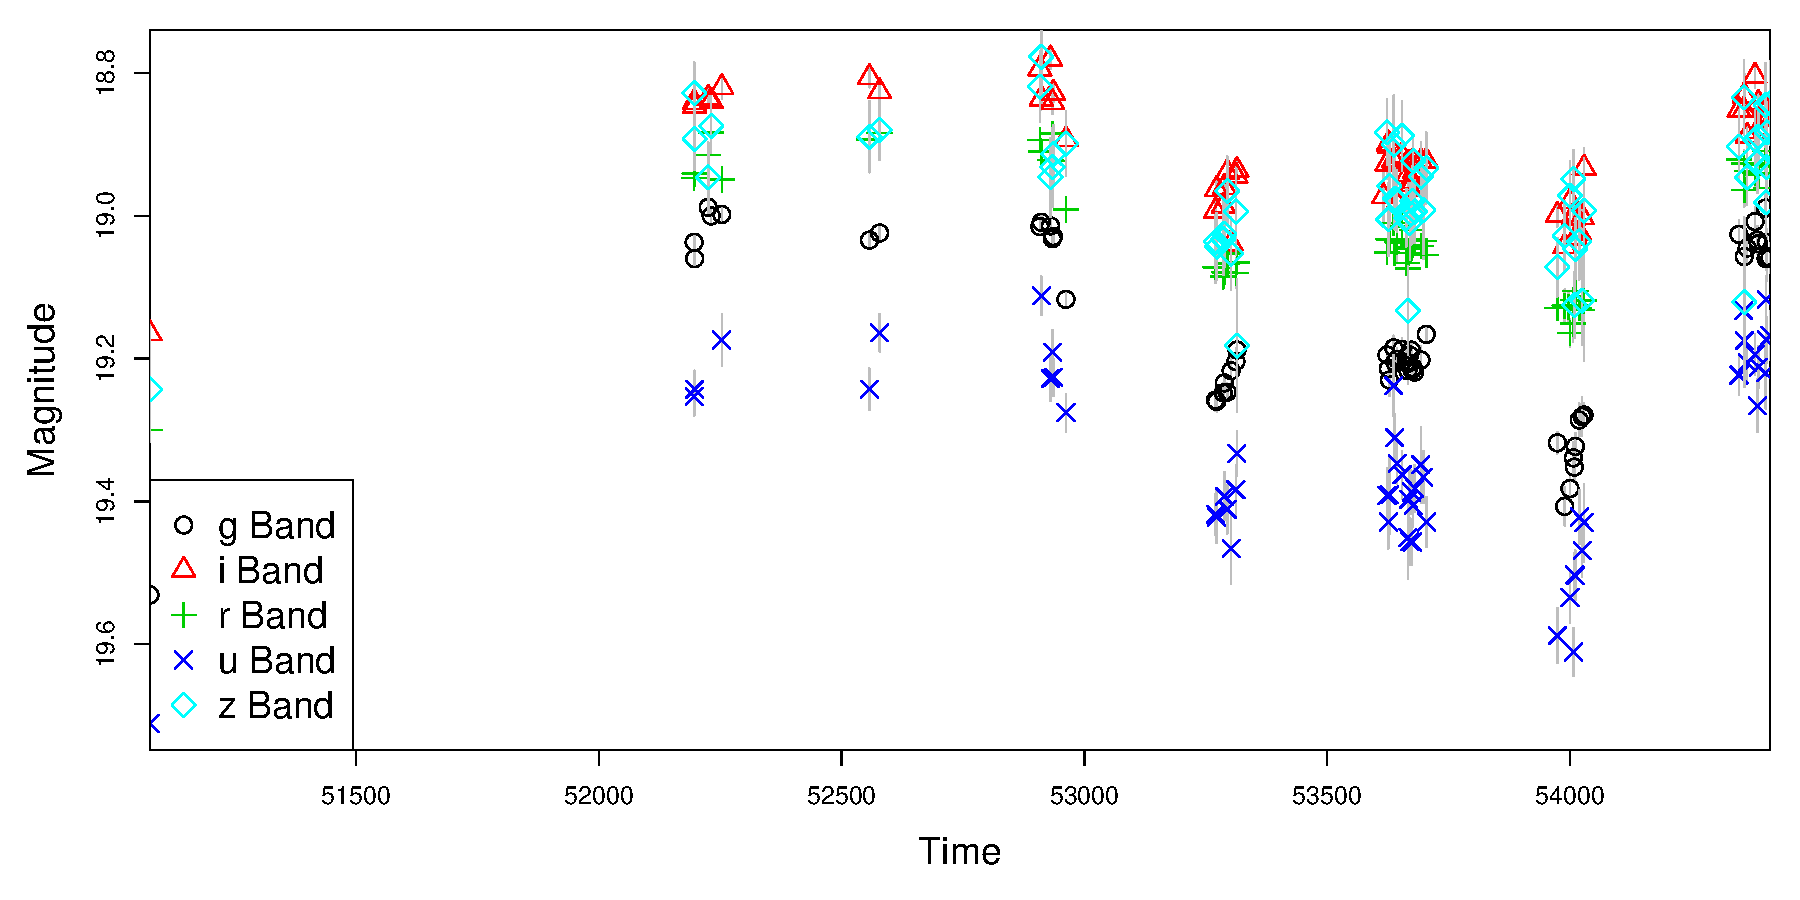
\includegraphics[scale=.15]{figs/unfolded_7904669.pdf}
\end{center}


\end{frame}


\begin{frame}{Example of Variable Star Science}
\begin{itemize}
\item For RR Lyrae variable stars distance is a function of mean brightness in $V$:
\begin{equation*}
d = 10^{(V-M_V +5)/5}
\end{equation*}
\item Discover structure in the Milky Way halo by \underline{identifying}, \underline{stimating distances} to RR Lyrae


\begin{center}
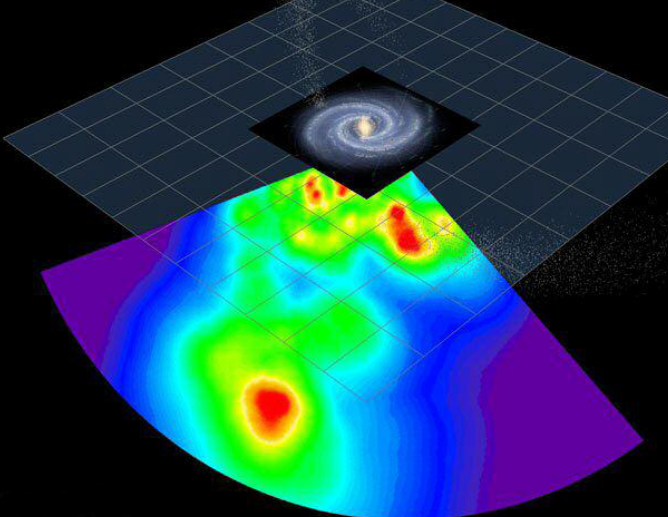
\includegraphics[scale=.2]{figs/sesar_map.png}\\
\footnotesize{Sesar \cite{sesar2010light} using SDSS Stripe 82 Data}
\end{center}

\item Compare observed structure to cosmological simulations.

\end{itemize}

\end{frame}



%% \begin{frame}{Mapping the Galactic Halo: Statistical Challenges}
%% \begin{itemize}
%% \item Classification: Identify RR Lyrae lightcurves.
%% \item Parametric Inference: Estimate periods, mean magnitudes, distances.
%% \item Nonparametric Inference: Construct 3--D density map.
%% \end{itemize}
%% \end{frame}


\begin{frame}{Mapping Galactic Halo with DES}

\textbf{Dark Energy Survey (DES)}
\begin{itemize}
\item 10 photometric measurements in ($g$,$i$,$r$,$z$,$Y$) over five years
\item depths to 24 mag in $i$
\item 5000 square degrees
\item few million variable stars
\end{itemize}

\vspace{.3in}

\begin{center}
DES is deeper and wider than SDSS Stripe 82, but much more sparsely sampled.
\end{center}

\end{frame}

%% \begin{frame}{Size of Variable Star Data Sets is Growing}
%% \begin{itemize}
%% \item \textit{Hipparcos} (1989--1993): 2712 
%% \item \textit{OGLE} (1992--present): 100,000s
%% \item \textit{DES} (ongoing): $\sim$ 10 million
%% \item \textit{LSST} (starting 2020): $\sim$ 1 billion

%% \vspace{.4in}

%% Data sets of varying quality:
%% \begin{center}
%% 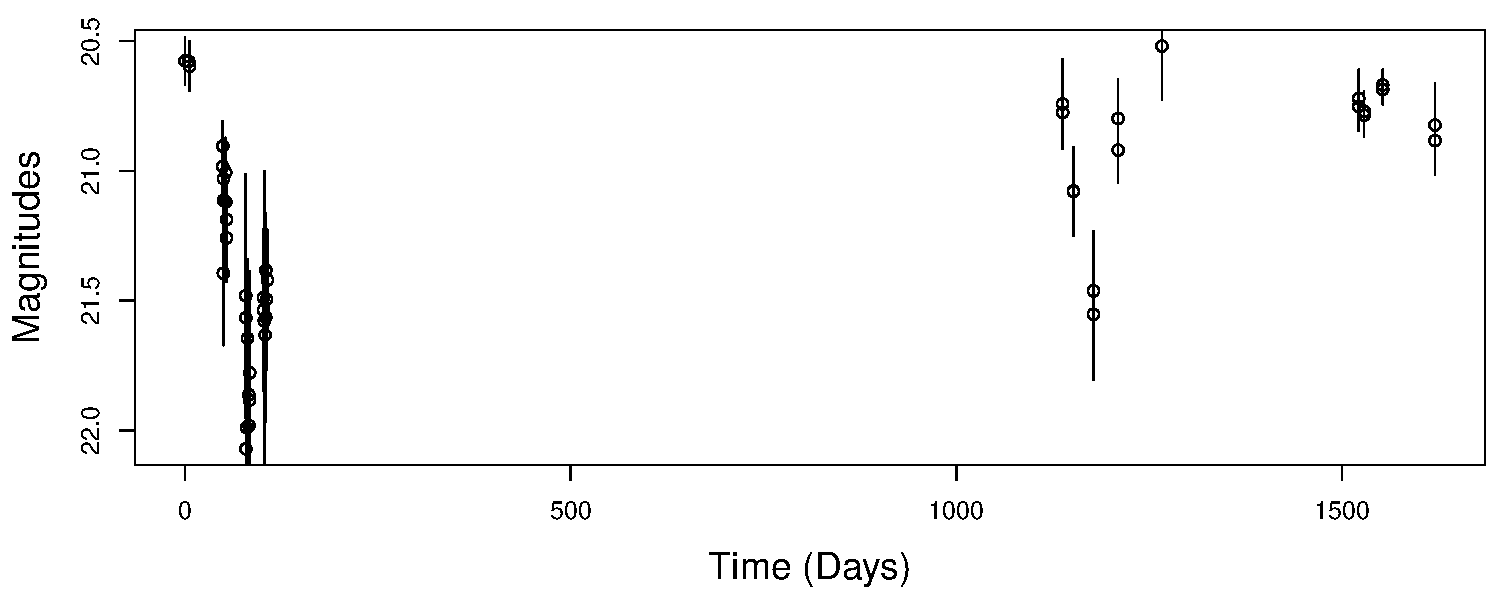
\includegraphics[scale=.3]{figs/m33_unfolded.pdf}
%% \end{center}


%% \end{itemize}

%% %\textbf{Dramatic Differences in Data Quality:}

%% \end{frame}



%% \section{Period Estimation Methods}



%% \begin{frame}{Sinusoid Based Models}

%% \textbf{Method:} Model light curve variation in each filter as sinusoid with $K$ harmonics. \cite{mondrik2015multiband,zechmeister2009generalised,lomb1976least,scargle1982studies,schwarzenberg1996fast}

%% \begin{equation*}
%% m_{jb} = \beta_b + \sum_{k=1}^K a_{bk}\sin(\omega t_{jb} + \phi_{bk}) + \epsilon_{jb}
%% \end{equation*}
%% where $\epsilon_{jb} \sim N(0,\sigma_{jb}^2)$.

%% \begin{itemize}
%% \item $(2K + 1)B + 1$ parameters. Pure sine $3B + 1$ parameters.
%% \item Maximum likelihood has closed form solution at fixed $\omega$
%% \begin{itemize}
%% \item Maximization strategy: Grid search on $\omega$.
%% \end{itemize}
%% \end{itemize}

%% \end{frame}


%% \begin{frame}{Example of Maximum Likelihood Fit with $K=2$}

%% \vspace{-.1in}

%% \begin{center}
%% 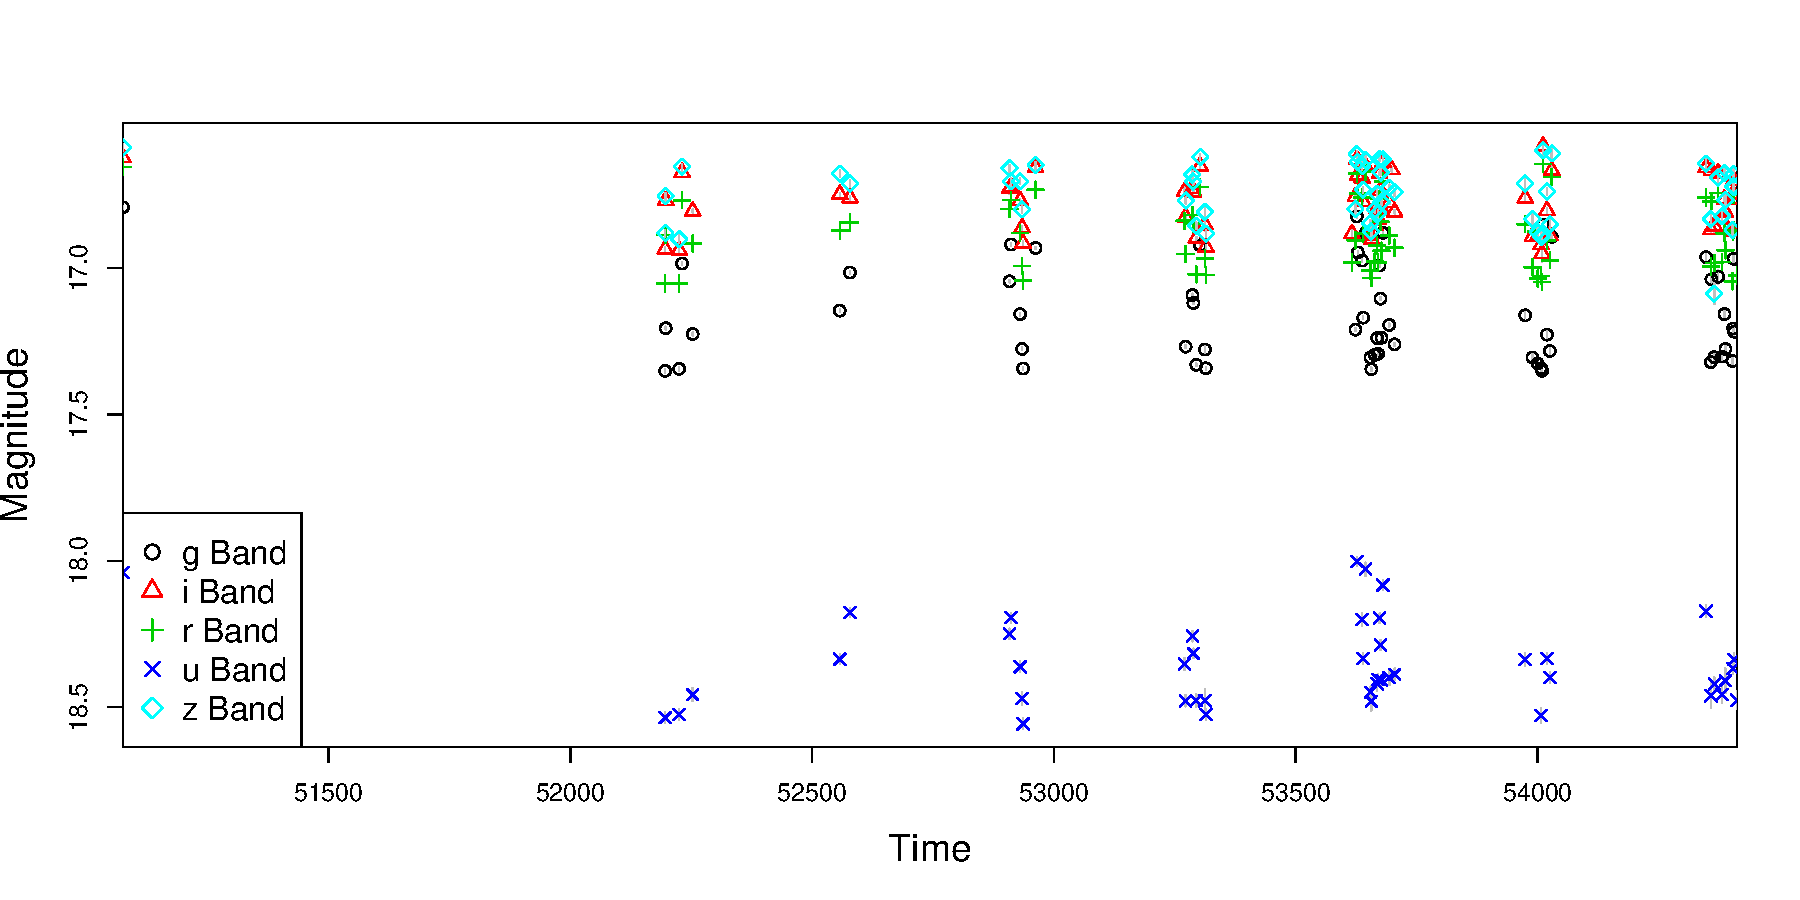
\includegraphics[scale=.25]{figs/rrlyrae_nomodel_fit.pdf}\\
%% 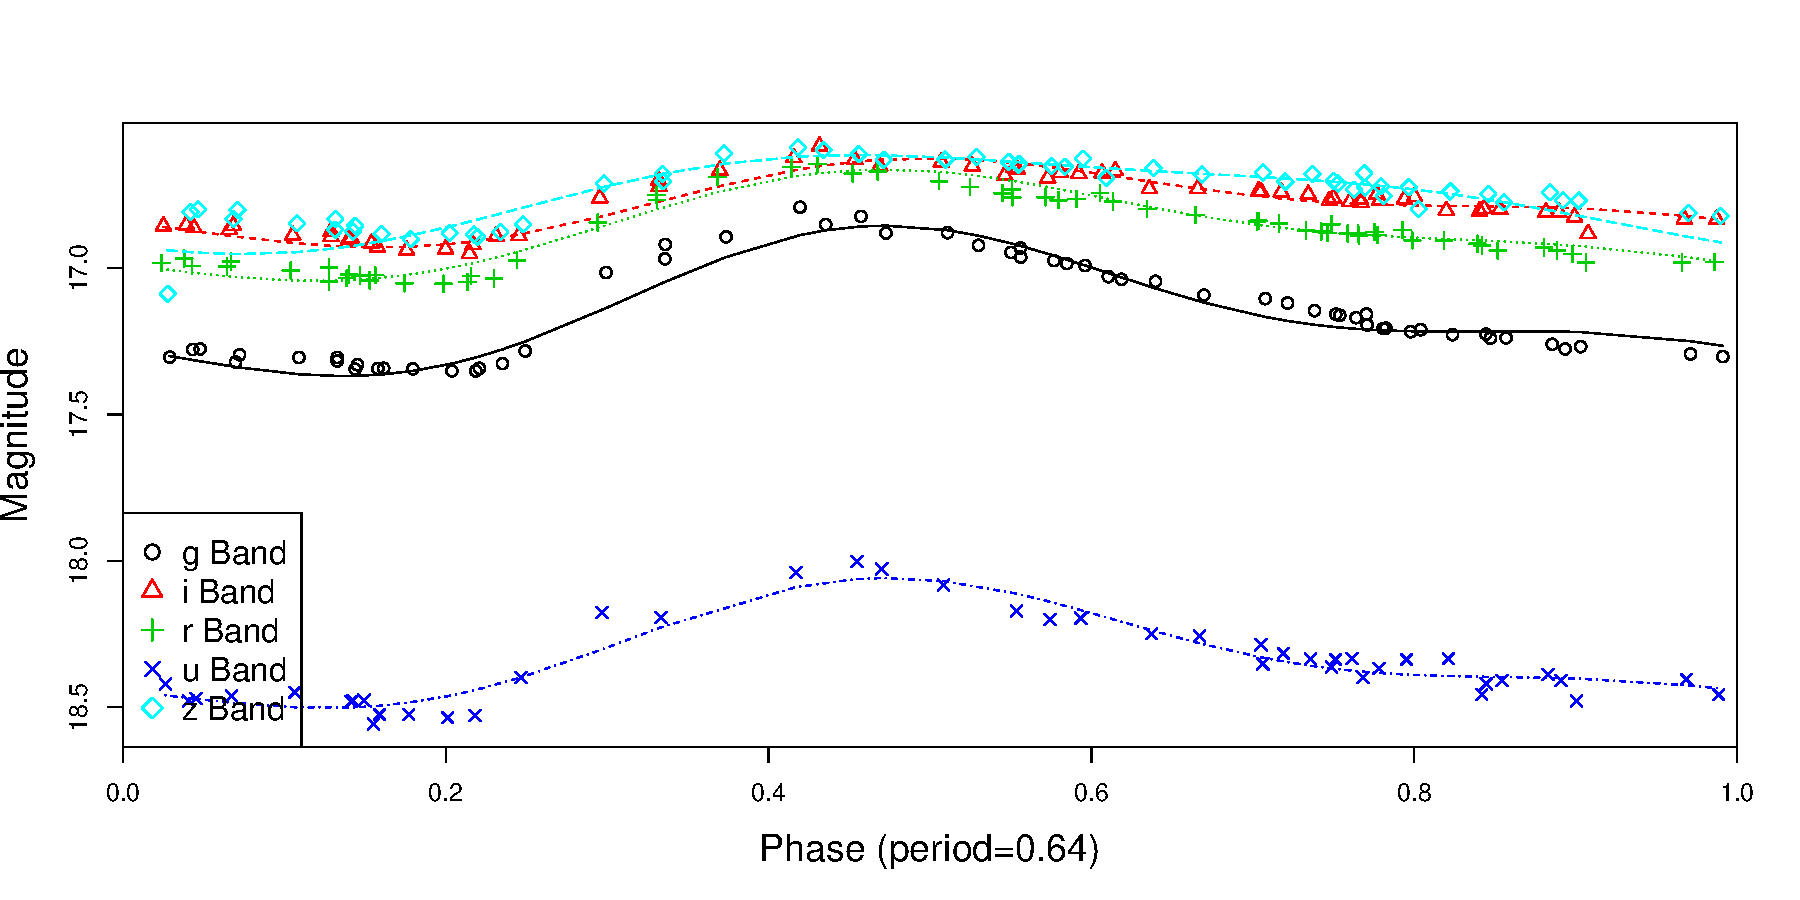
\includegraphics[scale=.25]{figs/rrlyrae_model_fit.pdf}\\
%% Total of $26$ parameters, model estimates period well.
%% \end{center}

%% \end{frame}

%% \begin{frame}{Output from Model Useful for Classification}

%% \begin{center}
%% 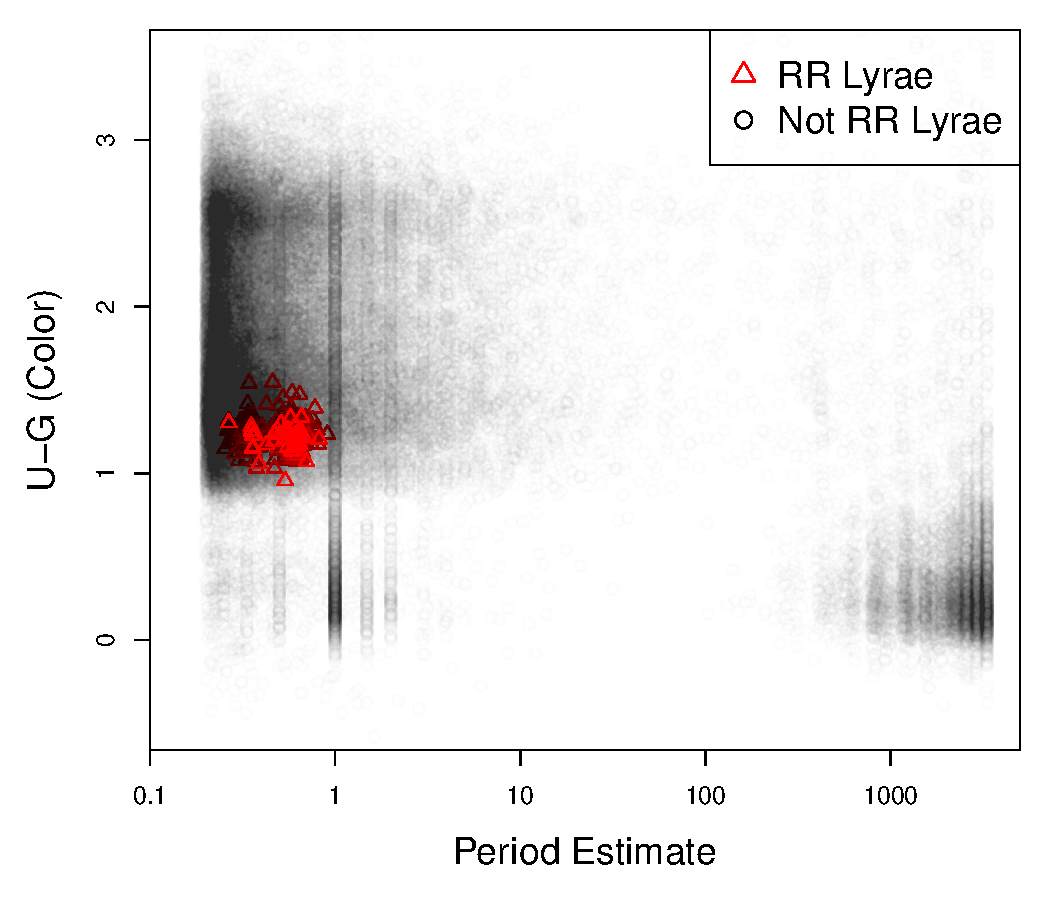
\includegraphics[scale=.4]{figs/sdss_color_period.pdf}
%% \end{center}


%% %%% TODO: make scatterplot of two features

%% \end{frame}


%% \begin{frame}{Problem: Sparsely Sampled Light Curves}


%% \begin{center}
%% 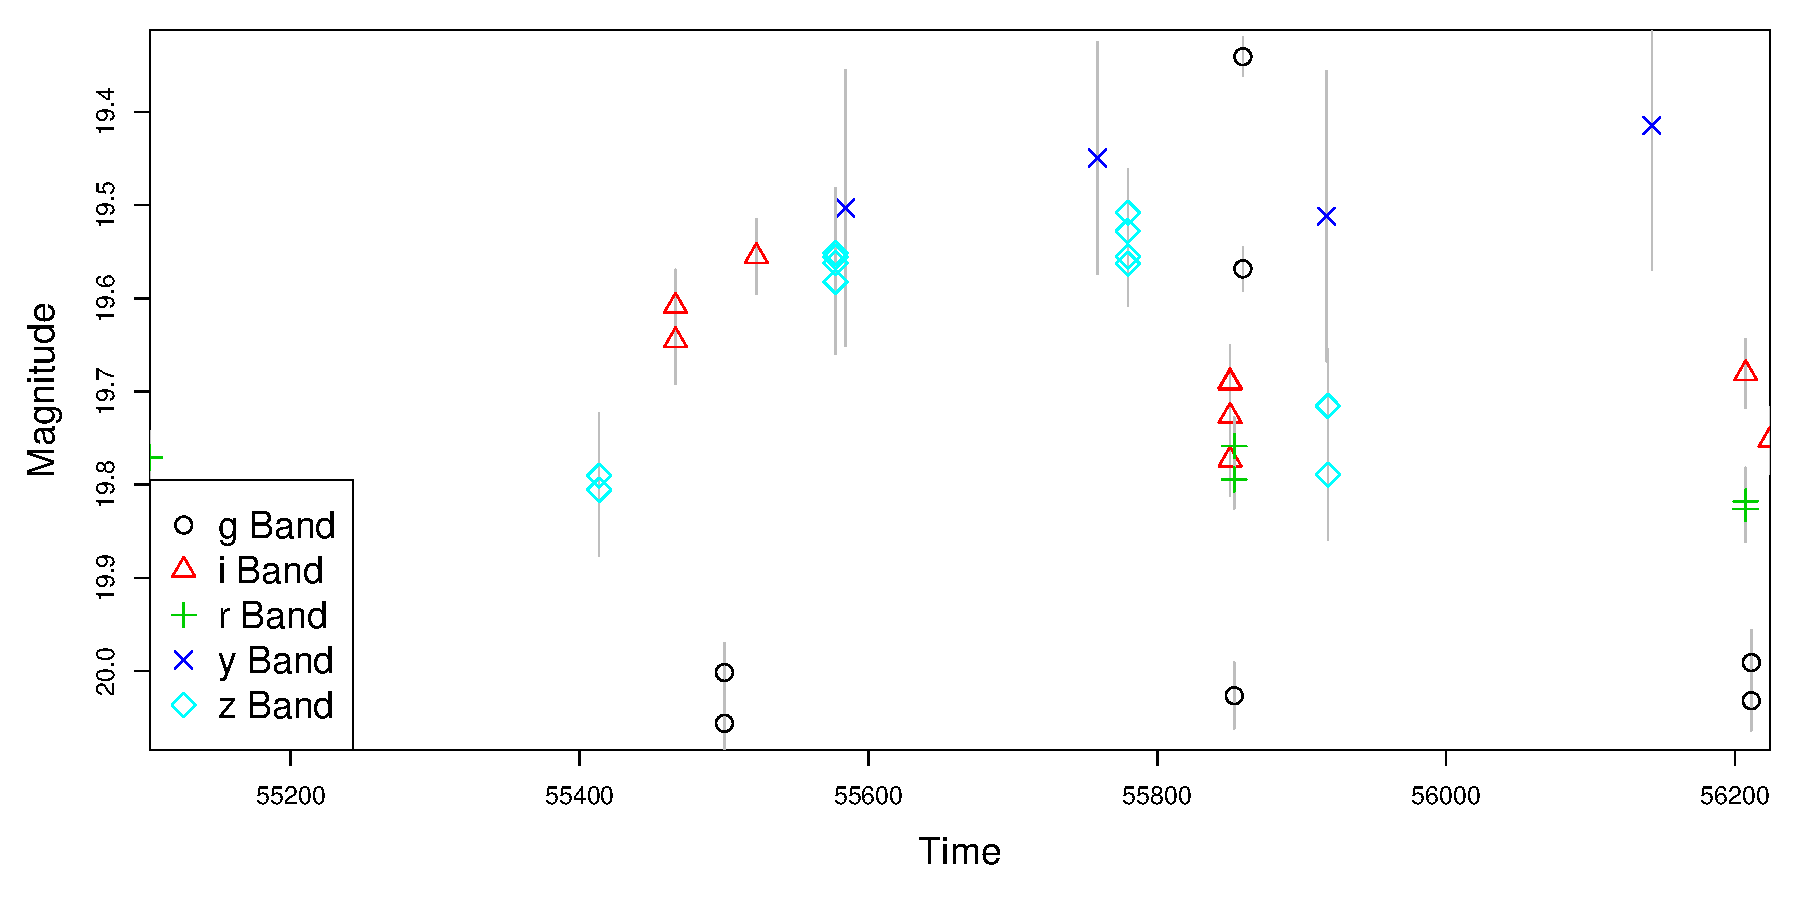
\includegraphics[scale=.3]{figs/unfolded_panstarrs.pdf}
%% \end{center}

%% \vspace{-.2in}

%% \begin{center}
%% \small{Pan--STARRS light curve. Period estimation difficult for this quality data.}
%% \end{center}


%% \end{frame}




%% \begin{frame}{Surveys Collecting Sparsely Sampled Light Curves}

%% \begin{itemize}
%% \item Dark Energy Survey (DES)
%% \begin{itemize}
%% \item 10 photometric measurements in ($g$,$i$,$r$,$z$,$Y$) over five years
%% \item depths to 24 mag in $i$
%% \item $\approx$ 100 million stars
%% \end{itemize}
%% \item Pan--STARRS
%% \end{itemize}
%% \end{frame}



%%%%%%%%
%%%%%%%% TODO: introduce model, discuss fitting
%%%%%%%%

\section{Classification and the Bias Variance Tradeoff}

\begin{frame}{Finding the RR Lyrae}

\end{frame}



\begin{frame}{Finding the RR Lyrae: Sesar 2010}

\end{frame}

\begin{frame}{Finding the RR Lyrae: Sesar 2010}

\end{frame}


\begin{frame}{Variance and Bias}
  \begin{itemize}
  \item \textbf{variance:} how much do my parameter estimates $\widehat{\theta}$ change if I ``perturb'' the data?
  \item \textbf{bias:}
  \item \textbf{tuning parameters:} parameters in a statistical method that are not of fundamental interest, but change output
  \item \textbf{variance--bias tradeoff:} tuning parameters ``negotiate'' a tradeoff between bias and variance to statistical procedures with good performance
  \item \textbf{cross validation:} one method for conducting this negotiation
  \end{itemize}

{\small Histogram binwidths.}
\end{frame}




\begin{frame}{Overview of Statistical Classification}

\textbf{Key Terms:}
\begin{itemize}
\item \textbf{training data:} lightcurves of known class
  \begin{itemize}
  \item eg SDSS Stripe 82 light curves (known RRL, not RRL)
  \end{itemize}
\item \textbf{unlabeled data:} lightcurves of unknown class
  \begin{itemize}
  \item eg DES variable sources
  \end{itemize}
\end{itemize}

\vspace{.2in}

\textbf{Steps in Classification:}
\begin{enumerate}
\item \textbf{feature extraction:} derive quantities from light curves useful for separating classes, eg period, amplitude, derivatives, etc.
\item \textbf{classifier construction:} using training data, construct function
\begin{equation*}
\widehat{\mathcal{C}}(features) \rightarrow class
\end{equation*} 
\item \textbf{apply classifier:} for unlabeled data, compute features and predict class using $\widehat{\mathcal{C}}$
\end{enumerate}
\end{frame}

\begin{frame}{Classification Problem with Two Features}
\begin{columns}[T] % align columns

\begin{column}{.5\textwidth}
%% \begin{center}
%% Training Data
%% \end{center}
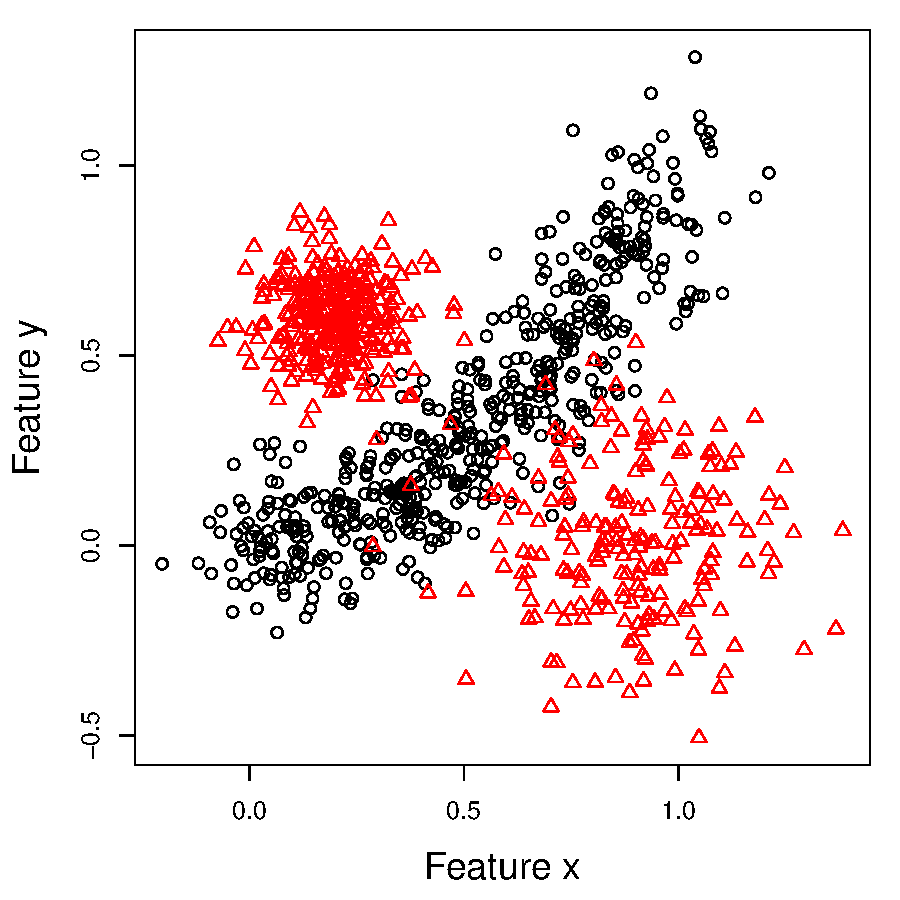
\includegraphics[height=2.3in,width=2.3in]{figs/sim_features.pdf}
\end{column}
\begin{column}{.5\textwidth}
  \begin{itemize}
  \item \textbf{dimension:} number of features
  \item with two features possible to make simple cuts
  \item harder with more than two features
  \item how do we assess error rate?
  \end{itemize}
\end{column}

\end{columns}

\end{frame}


\begin{frame}{Kernel Density Estimator}
  \begin{align*}
    p_k &= \text{probability an observation belongs to class } k\\
    f_k(x) &= \text{probability density of features for observations of class } k
  \end{align*}

\vspace{.2in}
  
  By Bayes theorem, the probability an observation with features $x$ belongs to class $k$ is
  \begin{equation*}
    p(k|x) = \frac{p_k f_k(x)}{\sum_{k=1}^K p_k f_k(x)}
  \end{equation*}

\textbf{Problem:} Do not know $p_k$ or $f_k$.  
\end{frame}



\begin{frame}{Kernel Density Estimator for Estimating $f_k$}

  \begin{equation*}
    \widehat{f}_k(x) = \frac{1}{\sum_{i=1}^n \ind_{z_i=k}}\sum_{i=1}^{n_k} K_h(x-x_i)\ind_{z_i=k}
  \end{equation*}

  \begin{itemize}
  \item $K_h(\cdot) = h^{-1}K(\cdot h^{-1})$
  \item $K$ is the kernel (often gaussian)
  \item $h$ is the bandwidth (tuning parameter)
  \end{itemize}

  \vspace{.3in}
  
  \begin{center}
    \textbf{The bandwidth plays the roll of binsize for histograms.}
  \end{center}

  \todo{write this in arbitrary dimension}
  
\end{frame}



\begin{frame}{The Bandwidth in 1 Dimension}

  \begin{center}
    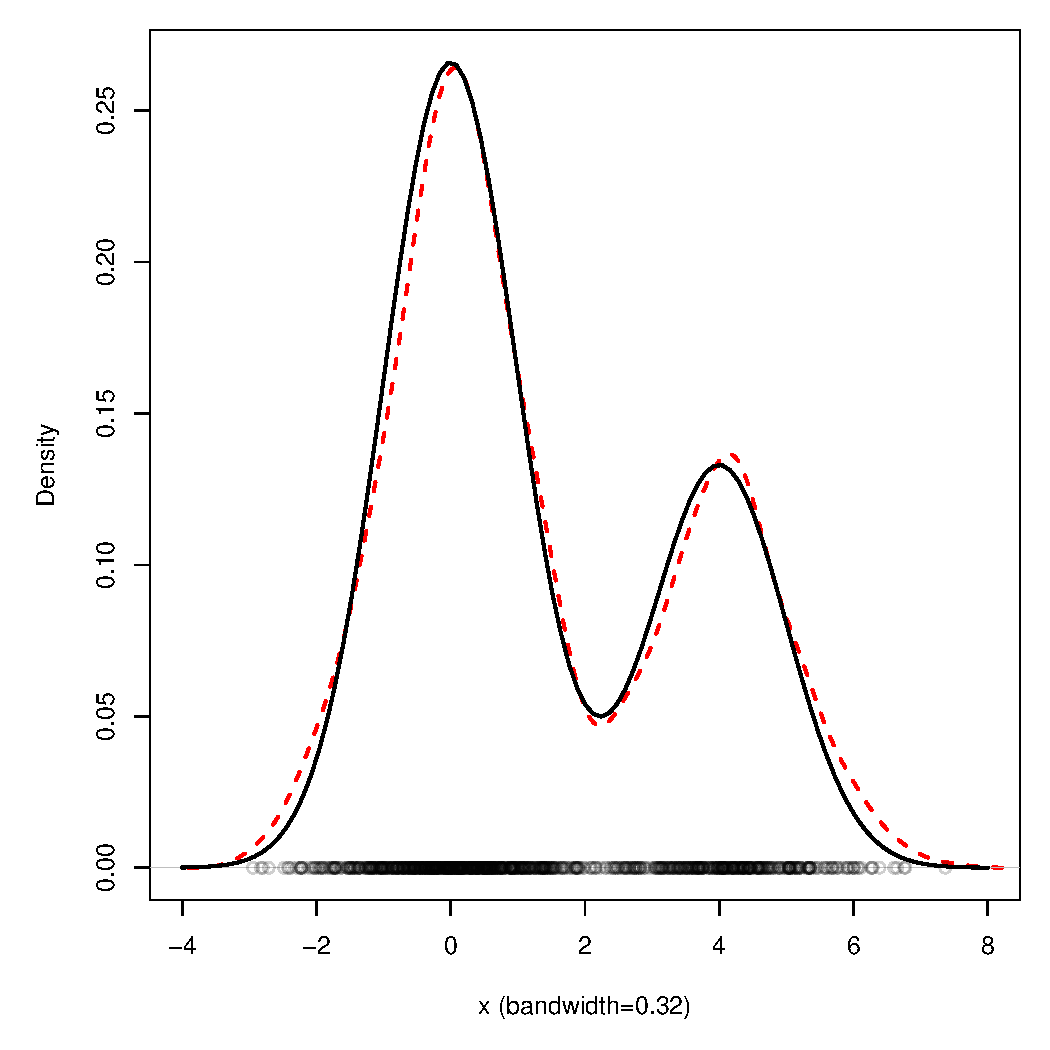
\includegraphics[scale=0.4]{figs/density2_1.pdf}
    \end{center}

\vspace{-.2in}
  
      \begin{center}
  The bandwidth looks appropriate.
      \end{center}
\end{frame}




\begin{frame}{The Bandwidth in 1 Dimension}


  \begin{center}
    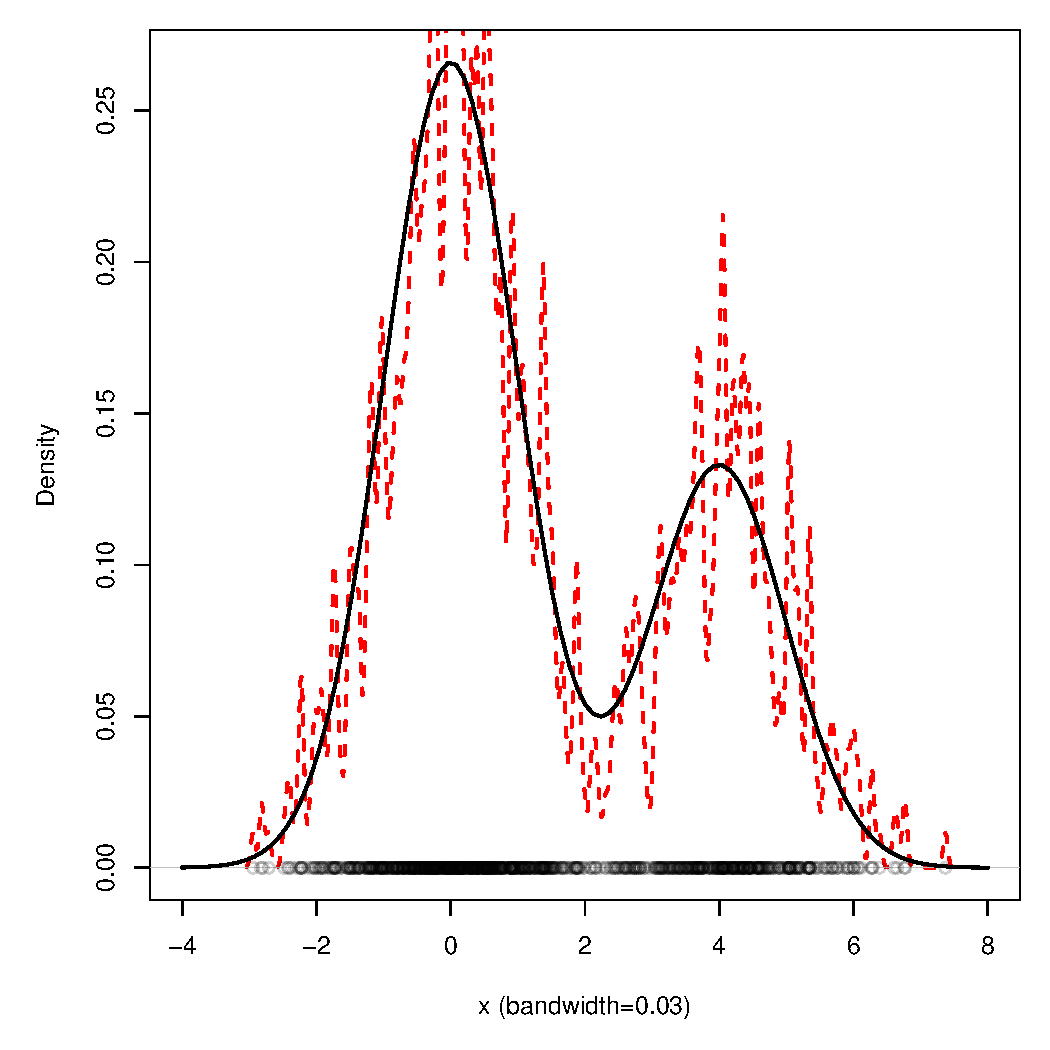
\includegraphics[scale=0.4]{figs/density1_1.pdf}
    \end{center}

\vspace{-.2in}

\begin{center}
    The bandwidth is too small, causing a large amount of \underline{variance} in estimator.
    \end{center}
  
\end{frame}



\begin{frame}{The Bandwidth in 1 Dimension}


  \begin{center}
    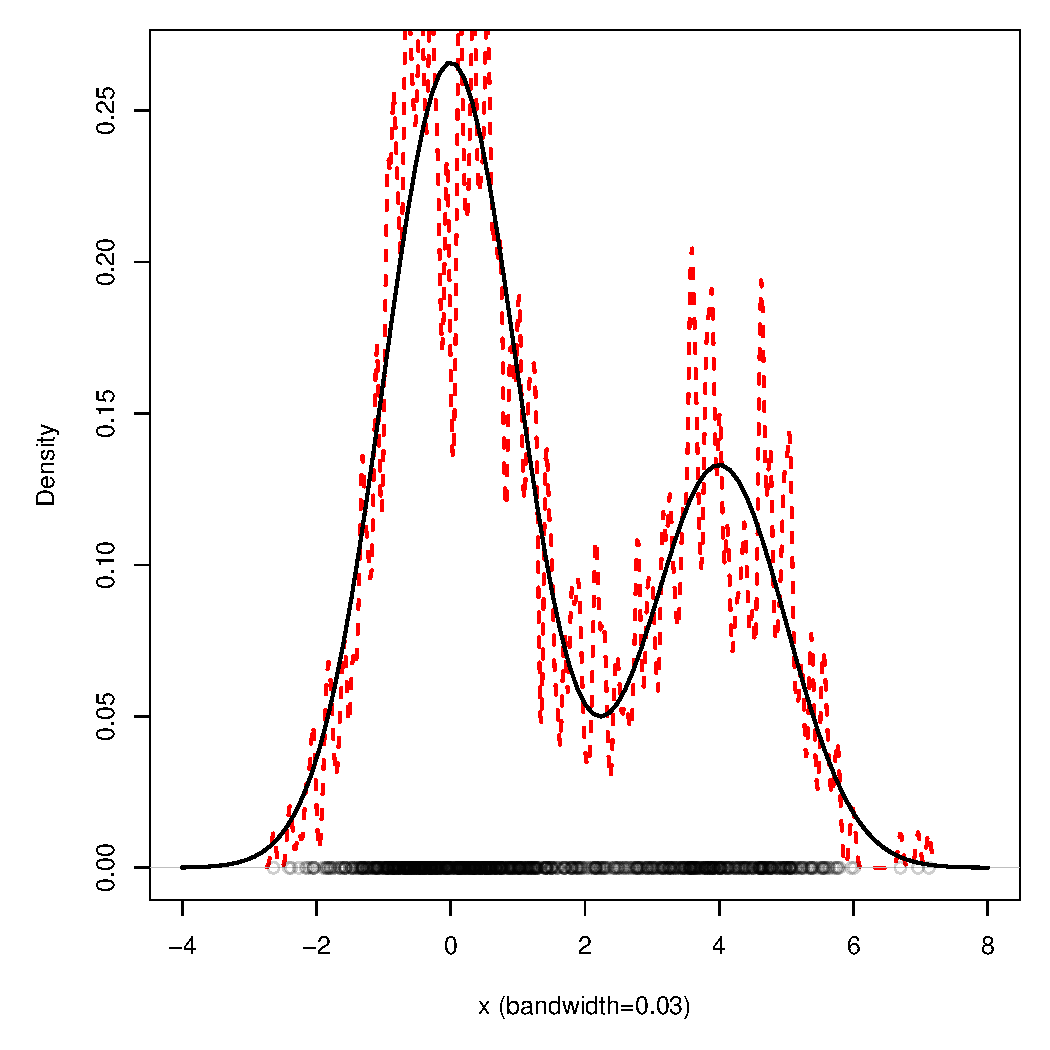
\includegraphics[scale=0.4]{figs/density1_2.pdf}
    \end{center}

\vspace{-.2in}

\begin{center}
  Same bandwidth, new data generated. The estimate has changed significantly ie high \underline{variance}.
\end{center}
  
\end{frame}



\begin{frame}{The Bandwidth in 1 Dimension}


  \begin{center}
    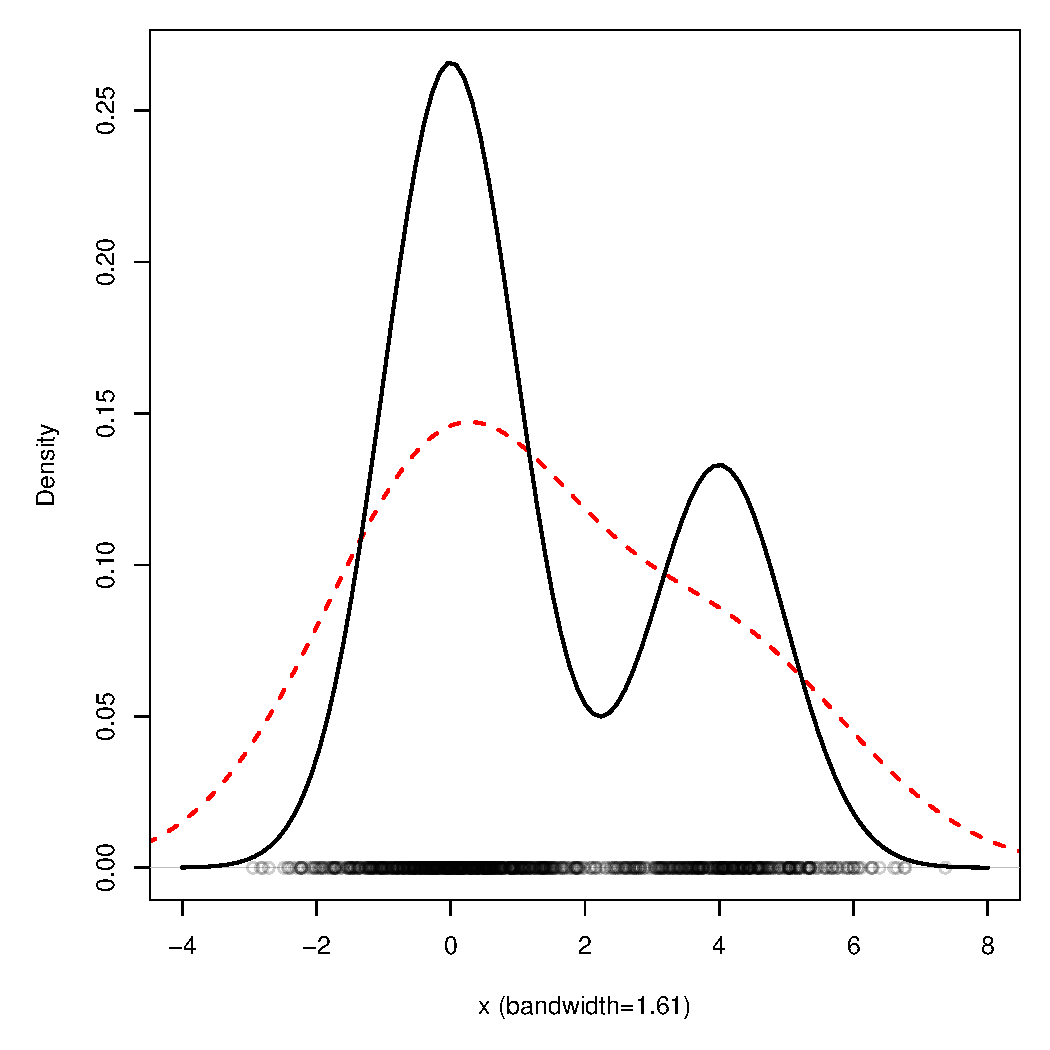
\includegraphics[scale=0.4]{figs/density3_1.pdf}
    \end{center}

\vspace{-.2in}

\begin{center}
  Bandwidth too large. Estimator is \underline{biased}.
\end{center}

  
\end{frame}



\begin{frame}{The Bandwidth in 1 Dimension}


  \begin{center}
    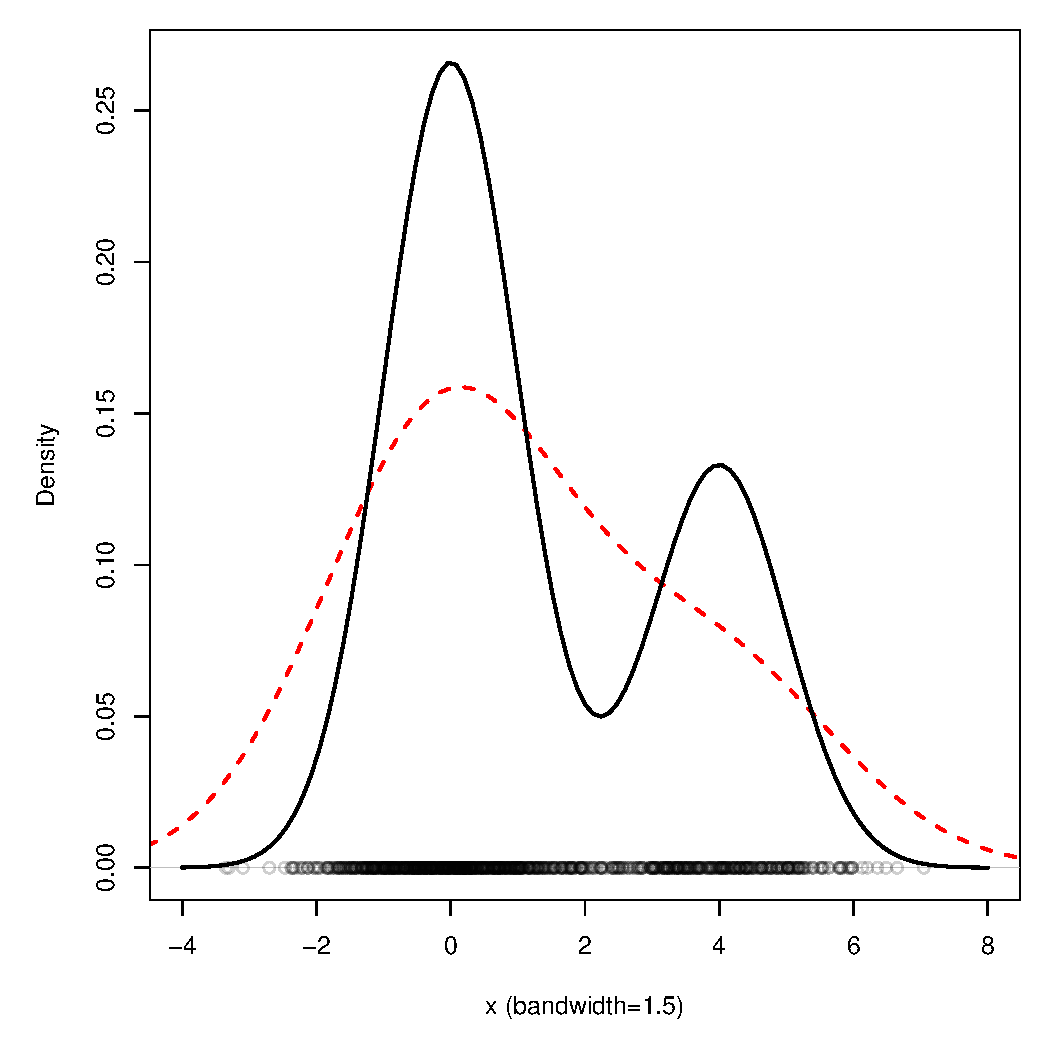
\includegraphics[scale=0.4]{figs/density3_2.pdf}
    \end{center}

\vspace{-.2in}

\begin{center}
  Same bandwidth, new data generated. Estimator looks the same, but \underline{biased}.
\end{center}

  
  
\end{frame}




\begin{frame}{Notes}
  \begin{itemize}
  \item ``sweet spot'' for bandwidth which balances variance--bias
  \item the best bandwidth depends on the sample size
    \begin{center}
      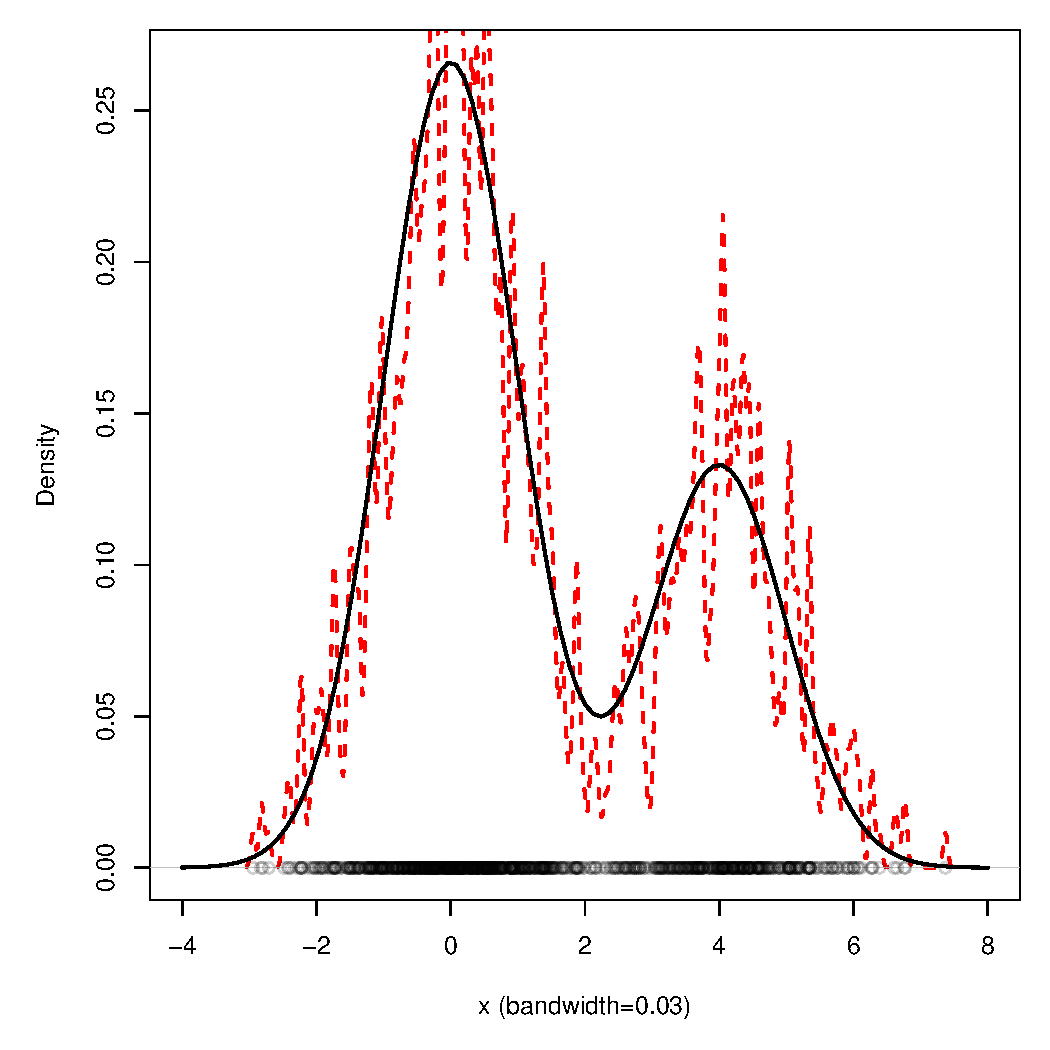
\includegraphics[scale=0.2]{figs/density1_1.pdf}
      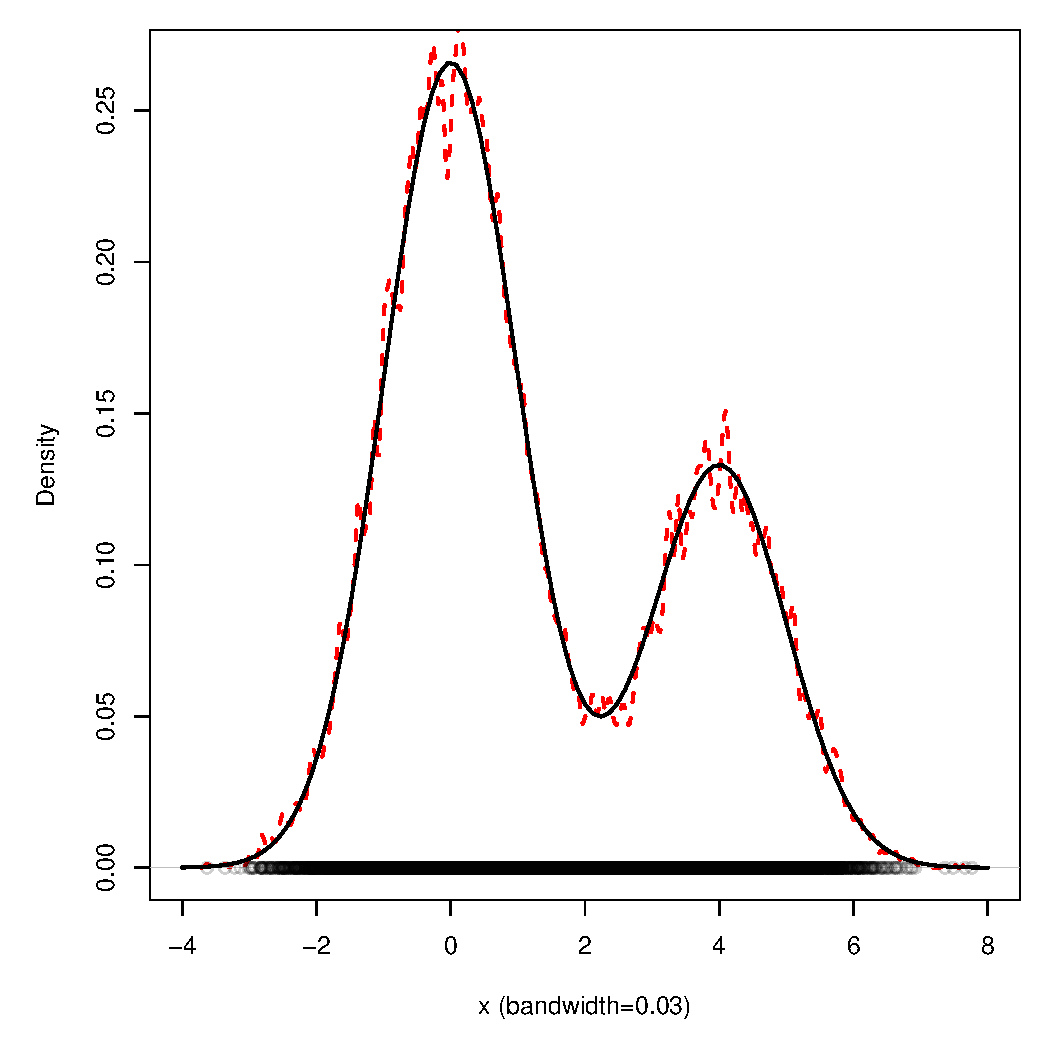
\includegraphics[scale=0.2]{figs/density1_largen.pdf}\\
      $a) bw=0.03, n = 1000 \, \, \, \, \,  \, \, \, \, b) bw=0.03, n=10000$
    \end{center}
  \item bandwidth lacks a clear interpretation
  \item bandwidth itself is not interesting
  \end{itemize}
\end{frame}





\begin{frame}{Back to Classification Example}

    \textbf{Message:} Too much variance. If I regenerated the data, the estiamte would completely change.
\end{frame}


\begin{frame}{Hueristic: Very Large Bandwidth}


  \textbf{Message:} Too much bias. The estimator is incapable of capturing important aspects in the density.
\end{frame}


\begin{frame}{Choosing the Bandwidth with Cross Valiation}

\end{frame}





\begin{frame}{Classifier Construction using CART}
\begin{columns}[T] % align columns

\begin{column}{.5\textwidth}
%% \begin{center}
%% Training Data
%% \end{center}
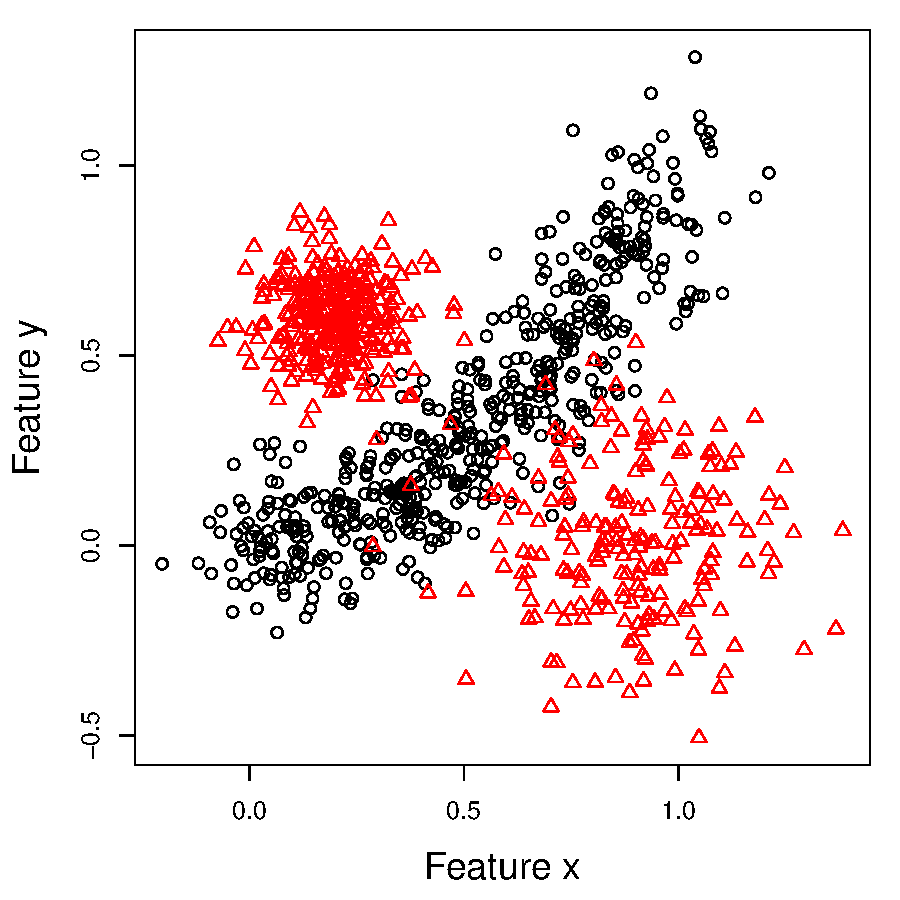
\includegraphics[height=2.3in,width=2.3in]{figs/sim_features.pdf}
\end{column}
\begin{column}{.5\textwidth}
\begin{itemize}
\item CART developed by Breiman et al in 1980's \cite{breiman1984classification}
\item recursively partitions feature space
\item partition represented by tree
\end{itemize}
\end{column}


\end{columns}
\end{frame}

\begin{frame}{Building CART Tree . . .}
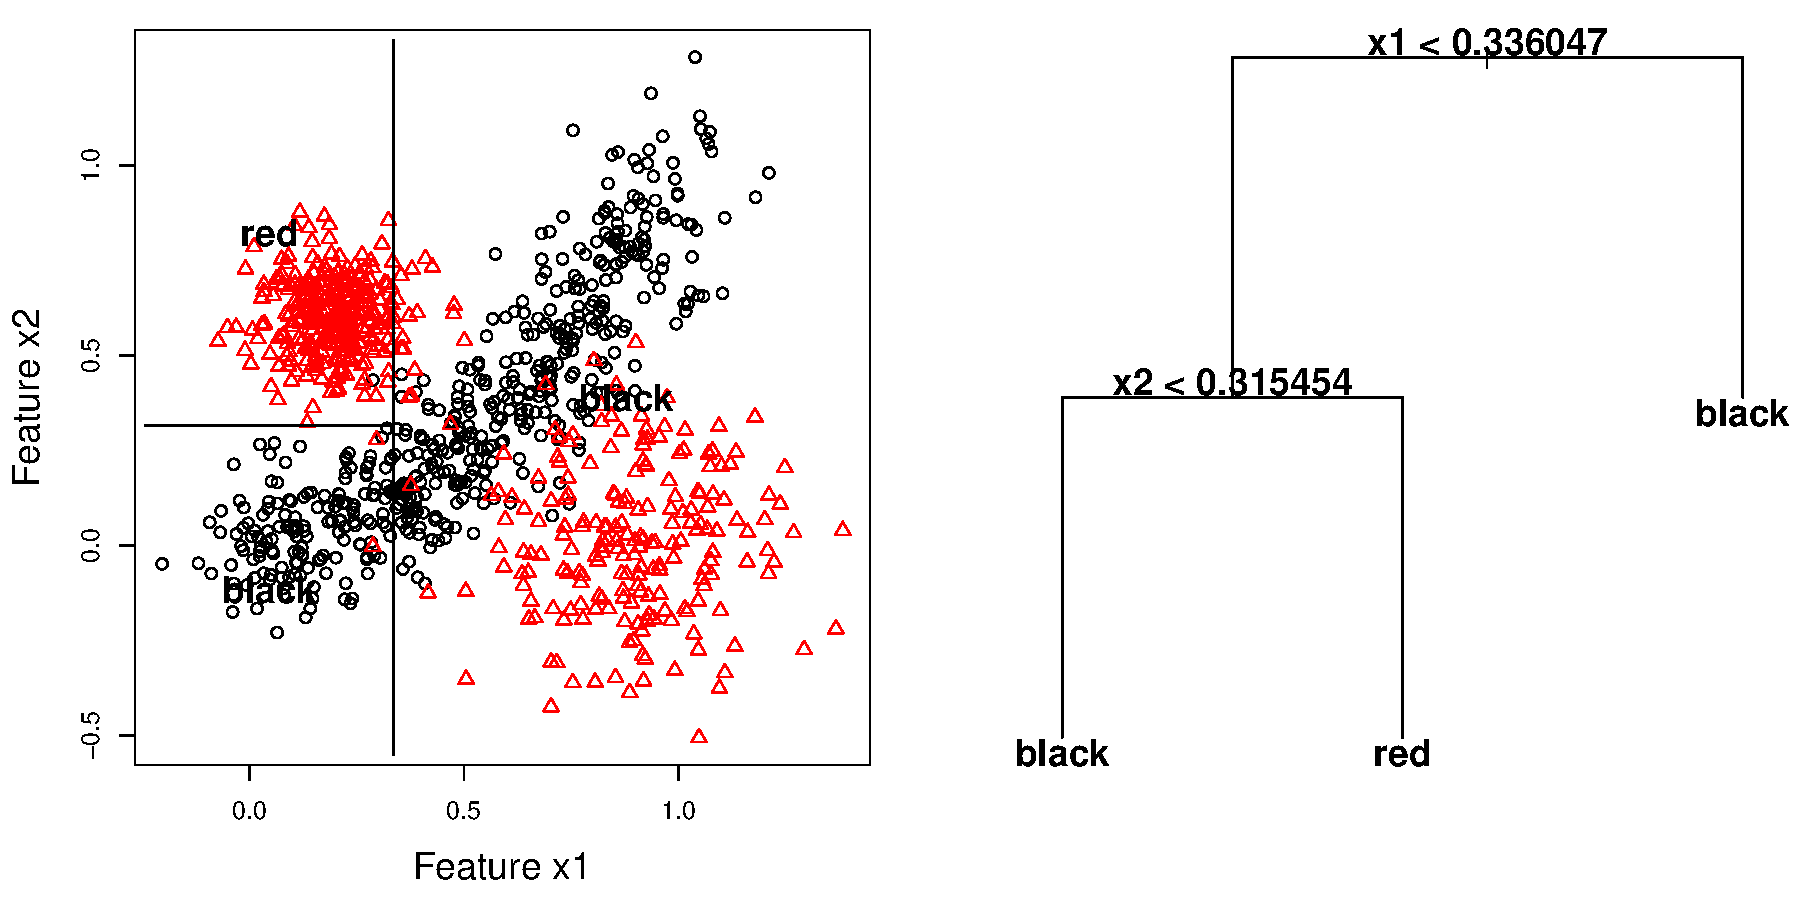
\includegraphics[height=2.3in,width=4.5in]{figs/tree_2.pdf}
\end{frame}

\begin{frame}{Building CART Tree . . .}
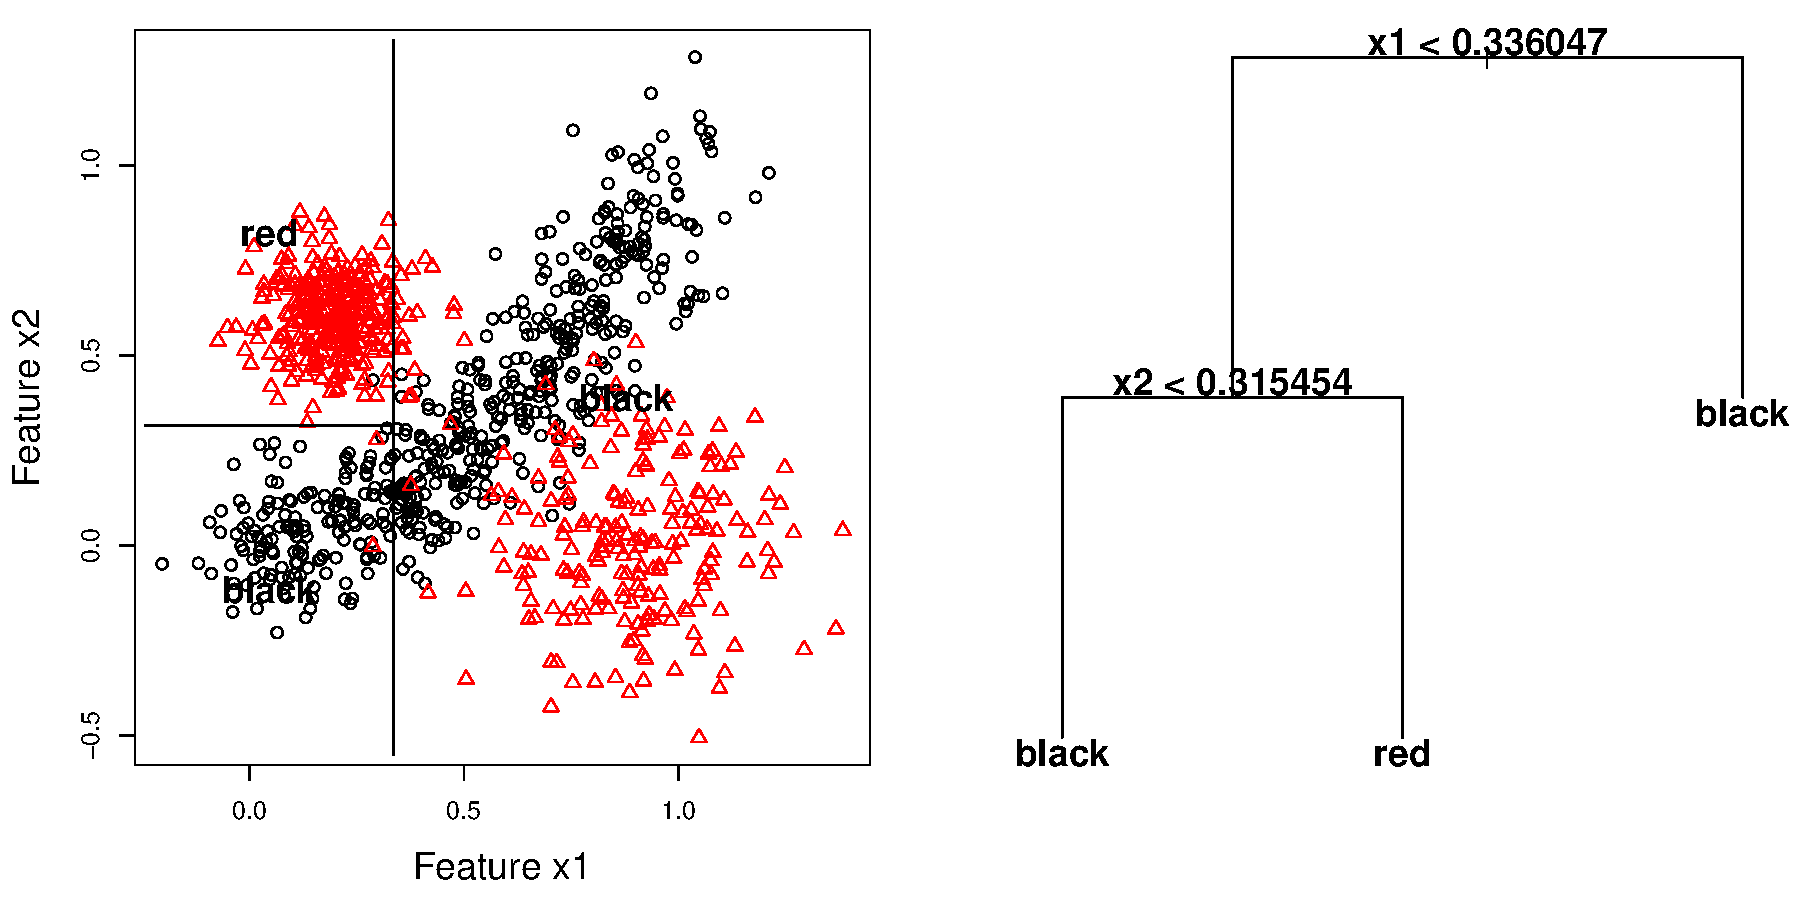
\includegraphics[height=2.3in,width=4.5in]{figs/tree_3.pdf}
\end{frame}

\begin{frame}{Building CART Tree . . .}
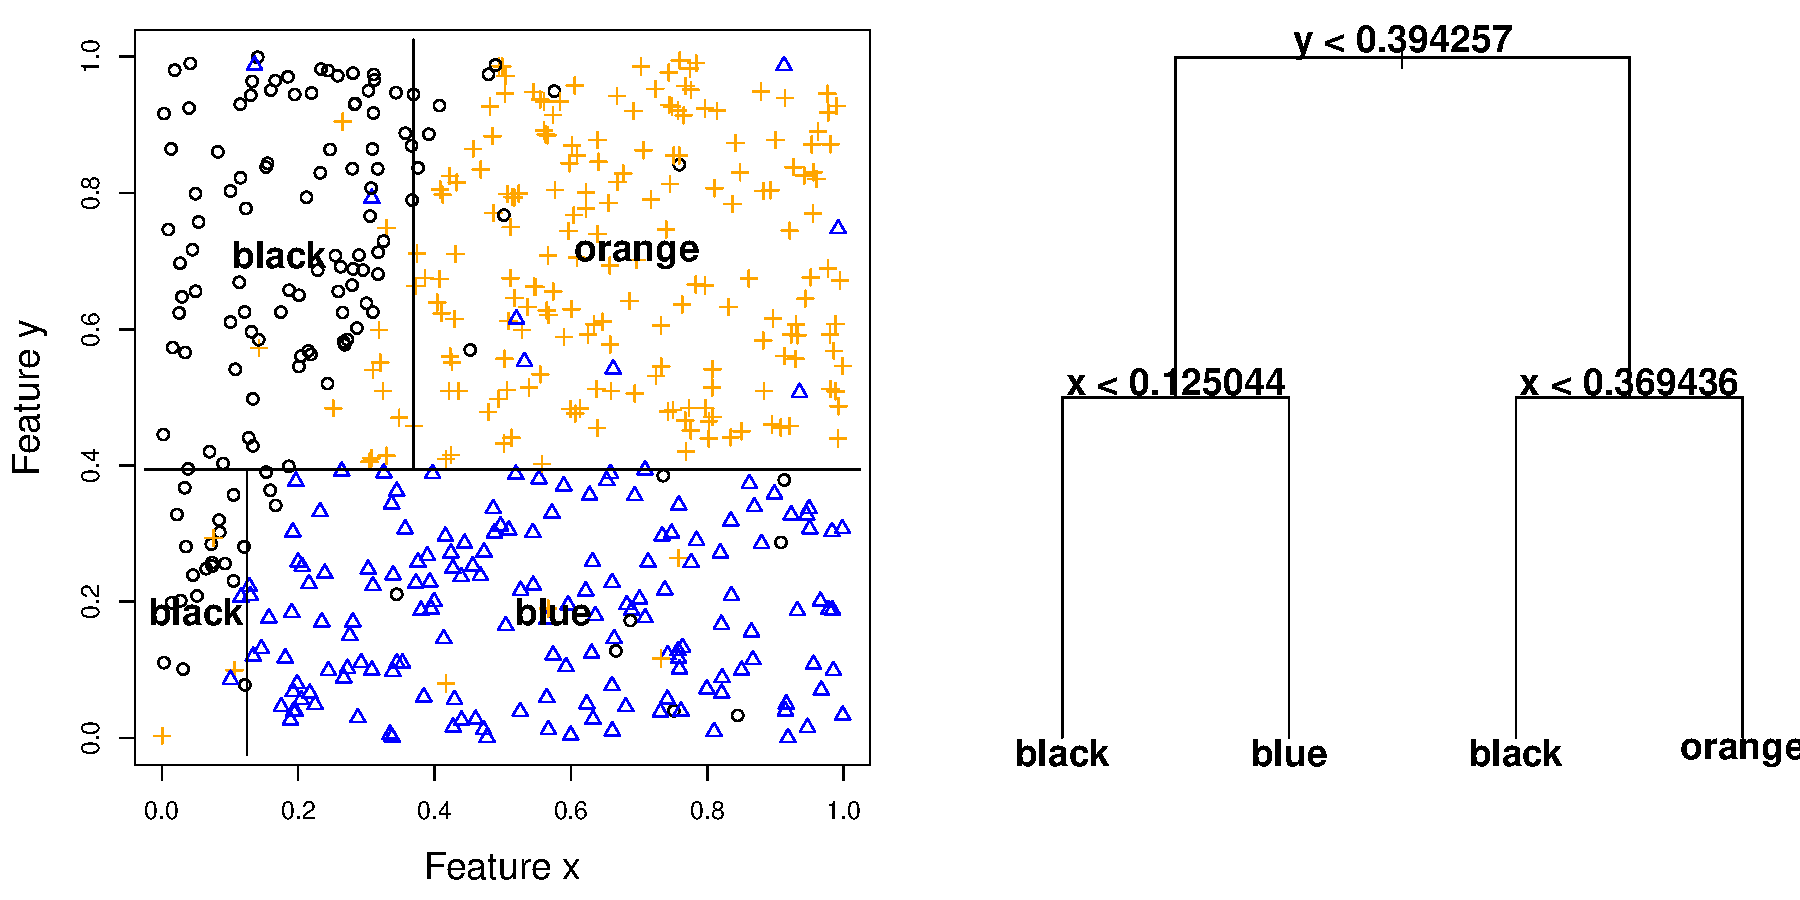
\includegraphics[height=2.3in,width=4.5in]{figs/tree_4.pdf}
\end{frame}

\begin{frame}{Resulting Classifier}
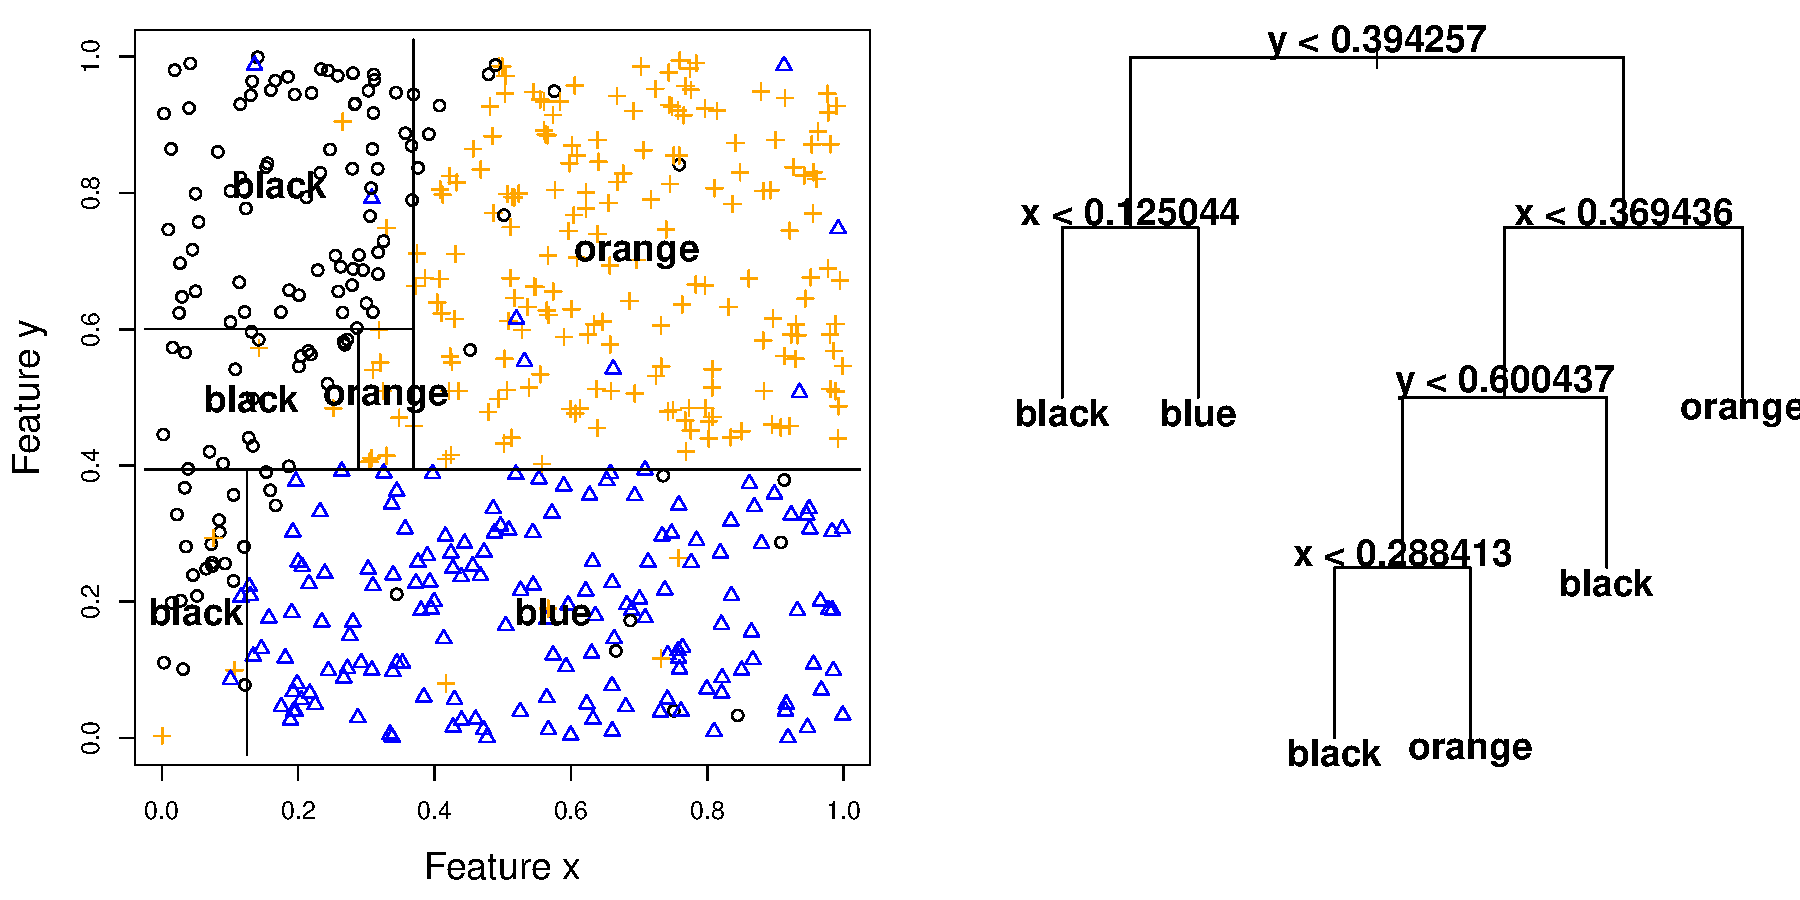
\includegraphics[height=2.3in,width=4.5in]{figs/tree_5.pdf}
\end{frame}

\begin{frame}{Apply Classifier to Test Data}

\textbf{Test Data:} Data used to evaluate classifier accuracy. Test data is not used to construct classifier.

\vspace{.1in}

\textbf{Confusion Matrix:} Rows are true class of test data. Columns are predicted class of test data. Entries are counts.

\vspace{.2in}

\begin{center}
\begin{tabular}{lccc}
\hline
 & \multicolumn{3}{c}{Predicted} \\ 
Truth  & black & blue & \multicolumn{1}{c}{orange} \\ 
\hline
black  & $23$ & $\phantom{0}1$ & $\phantom{0}7$ \\
blue  & $\phantom{0}2$ & $30$ & $\phantom{0}2$ \\
orange  & $\phantom{0}3$ & $\phantom{0}1$ & $31$ \\
\hline 
\end{tabular}

\end{center}

\end{frame}


\begin{frame}{Notes}
  \begin{itemize}
  \item the kernel density estimator is a smooth version of a histogram
    \begin{itemize}
    \item bandwidth of kde $\leftrightarrow$ bin width of histogram
    \end{itemize}
  \item classifiers have strengths and weaknesses
    \begin{itemize}
    \item kde works well in low dimension with a lot of data
    \item CART works in moderate dimensions with nonlinear decision boundaries
    \end{itemize}
  \item many other types of classifiers: support vector machines, random forests, neural networks
    \begin{itemize}
    \item some of the more advanced methods automatically balance bias--variance tradeoff
    \end{itemize}
  \end{itemize}
\end{frame}


%% \begin{frame}{Notes on CART}
%% \begin{itemize}
%% \item Nearly always have $>2$ features.
%% \item Number of splits in tree is chosen by pruning.
%% \item CART is moderately good classifier from accuracy perspective.
%% \item CART is basis for more accurate / sophisticated classifiers such as Random Forest.
%% \end{itemize}
%% \end{frame}



\section{Parameter Estimation for Sparsely Sampled Variable Stars}

%% \begin{frame}{Parsimonious RR Lyrae Model}

%% \underline{global parameters} common for all RR Lyrae:
%% {\footnotesize
%% \begin{align*}
%% M_b &=  \text{ absolute magnitude band $b$ }\\
%% R_b &= \text{ attenuation caused by dust in band $b$ }\\
%% \gamma_b &= \text{ normalized shape of light curve in band $b$ }\\
%% \end{align*}
%% }

%% \vspace{.2in}

%% \begin{equation*}
%% m_b(t) = \mu + M_b + E[B-V]R_b + a\gamma_b(\omega t + \phi)
%% \end{equation*}

%% \vspace{.2in}

%% \underline{individual parameters} specific to each RR Lyrae:
%% {\footnotesize
%% \begin{align*}
%% \mu &= \text{ distance modulus }\\
%% E[B-V] &= \text{ amount of dust }\\
%% a &= \text{ amplitude of variation }\\
%% \omega &= \text{ frequency of variation }\\
%% \phi &= \text{ phase }
%% \end{align*}
%% }

%% \end{frame}


\begin{frame}{Period Estimation Methods}

\end{frame}


\begin{frame}{More on Period Estimation Methods}

\end{frame}


\begin{frame}{Do Not Work for Sparsely Sampled Light Curves}

\end{frame}


\begin{frame}{Template Based Methods}

\end{frame}


\begin{frame}{Parsimonious RR Lyrae Model}


\begin{center}
global parameters fit once for all RR Lyrae\\
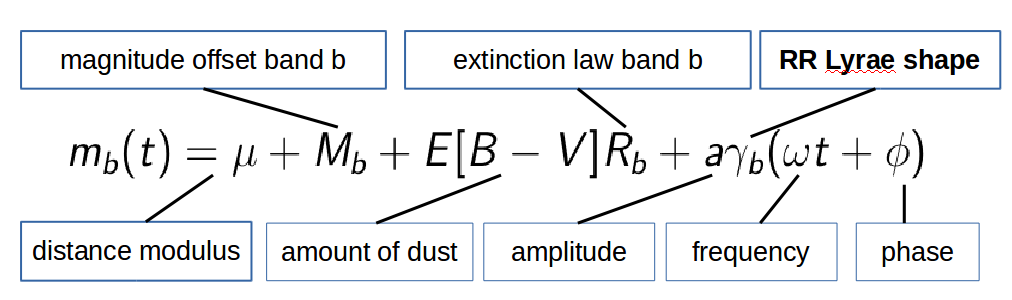
\includegraphics[scale=.3]{figs/model.png}\\
individual parameters fit for each RR Lyrae
\end{center}

\vspace{.2in}

\begin{itemize}
\item Data $D=\{\{t_{jb},m_{jb},\sigma_{jb}\}_{j=1}^{n_b}\}_{b=1}^B$
\item Normal measurement error model:
\begin{equation*}
m_{jb} = m_b(t_{jb}) + \epsilon_{jb}
\end{equation*}
where $\epsilon_{jb} \sim N(0,\sigma_{jb}^2)$.
\end{itemize}
\end{frame}

\begin{frame}{$\gamma_b$ Estimated from SDSS Stripe 82 RR Lyrae}

\begin{center}
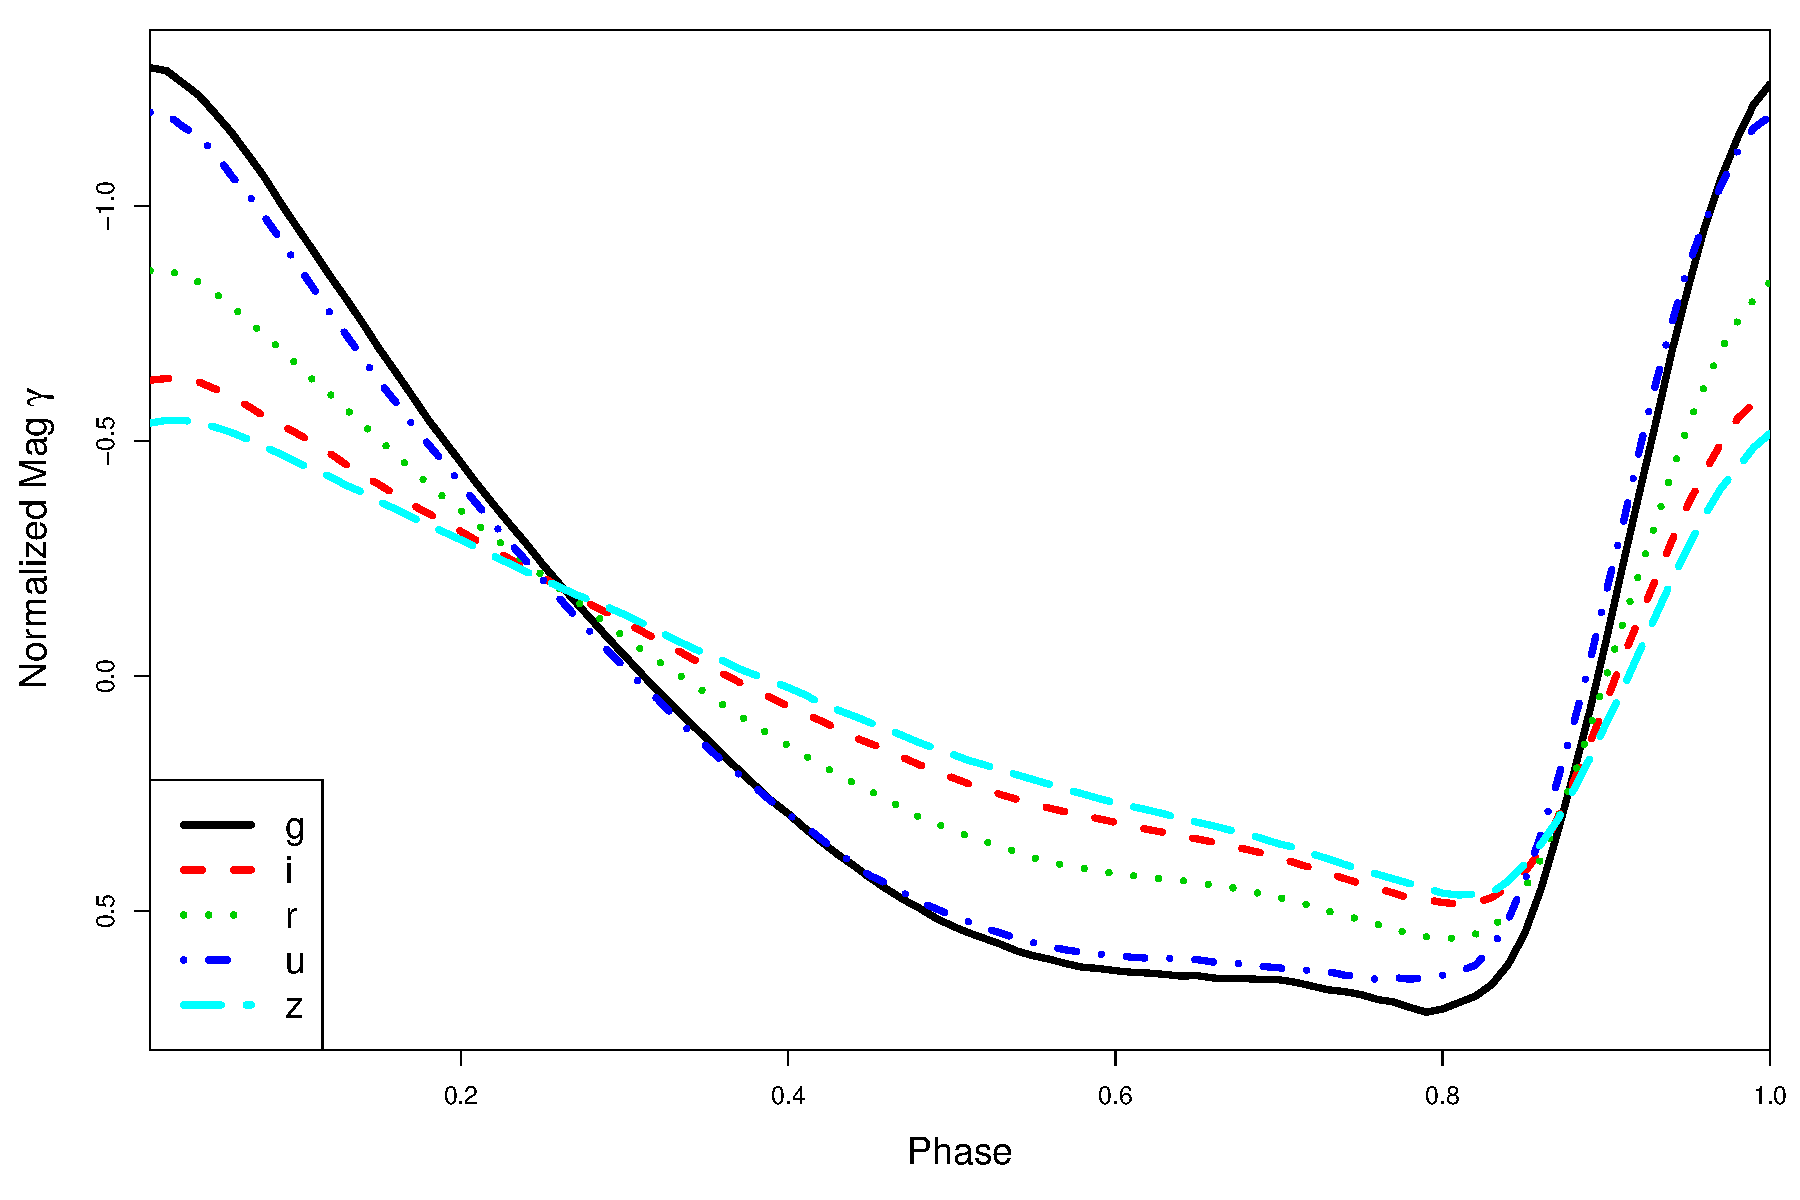
\includegraphics[scale=.3]{figs/templates.pdf}
\end{center}

\end{frame}

\begin{frame}{Parameter Estimation}
%%\begin{itemize}
%% \item Likelihood:
%% \begin{equation*}
%% m_{jb} = m_b(t_{jb}) + \epsilon_{jb} 
%% \end{equation*}
%% where $\epsilon_{jb} \sim N(0,\sigma_{jb}^2)$.
%% \item Define
%% \begin{align*}
%% &RSS(\omega,\mu,E[B-V],a,\phi) \\
%%  &\equiv\sum_{b=1}^B \sum_{j=1}^{n_b}\left(\frac{m_{jb} - \mu - M_b - E[B-V]R_b - a\gamma_b(\omega t_{jb} + \phi)}{\sigma_{bi}}\right)^2
%% \end{align*}
%% \end{itemize}
\begin{align*}
&RSS(\omega,\mu,E[B-V],a,\phi) \\
 &\equiv\sum_{b=1}^B \sum_{j=1}^{n_b}\left(\frac{m_{jb} - \mu - M_b - E[B-V]R_b - a\gamma_b(\omega t_{jb} + \phi)}{\sigma_{jb}}\right)^2
\end{align*}


Estimate parameters with maximum likelihood ($\chi^2$ minimization):
\begin{itemize}
\item Likelihood is highly multimodal in $\omega$, grid search.
\item Model is linear in $\mu$,$E[B-V]$, and $a$, closed form updates.
\item Warm start Newton--Raphson updates for $\phi$.
\end{itemize}

\end{frame}

\section{Simulation Results}

\begin{frame}{Simulation}

  \begin{textblock*}{12cm}(.5cm,2cm) % {block width} (coords)
Downsample Stripe 82 variables to 20 observations across all bands:
\end{textblock*}

  \begin{textblock*}{3cm}(1cm,3.1cm) % {block width} (coords)
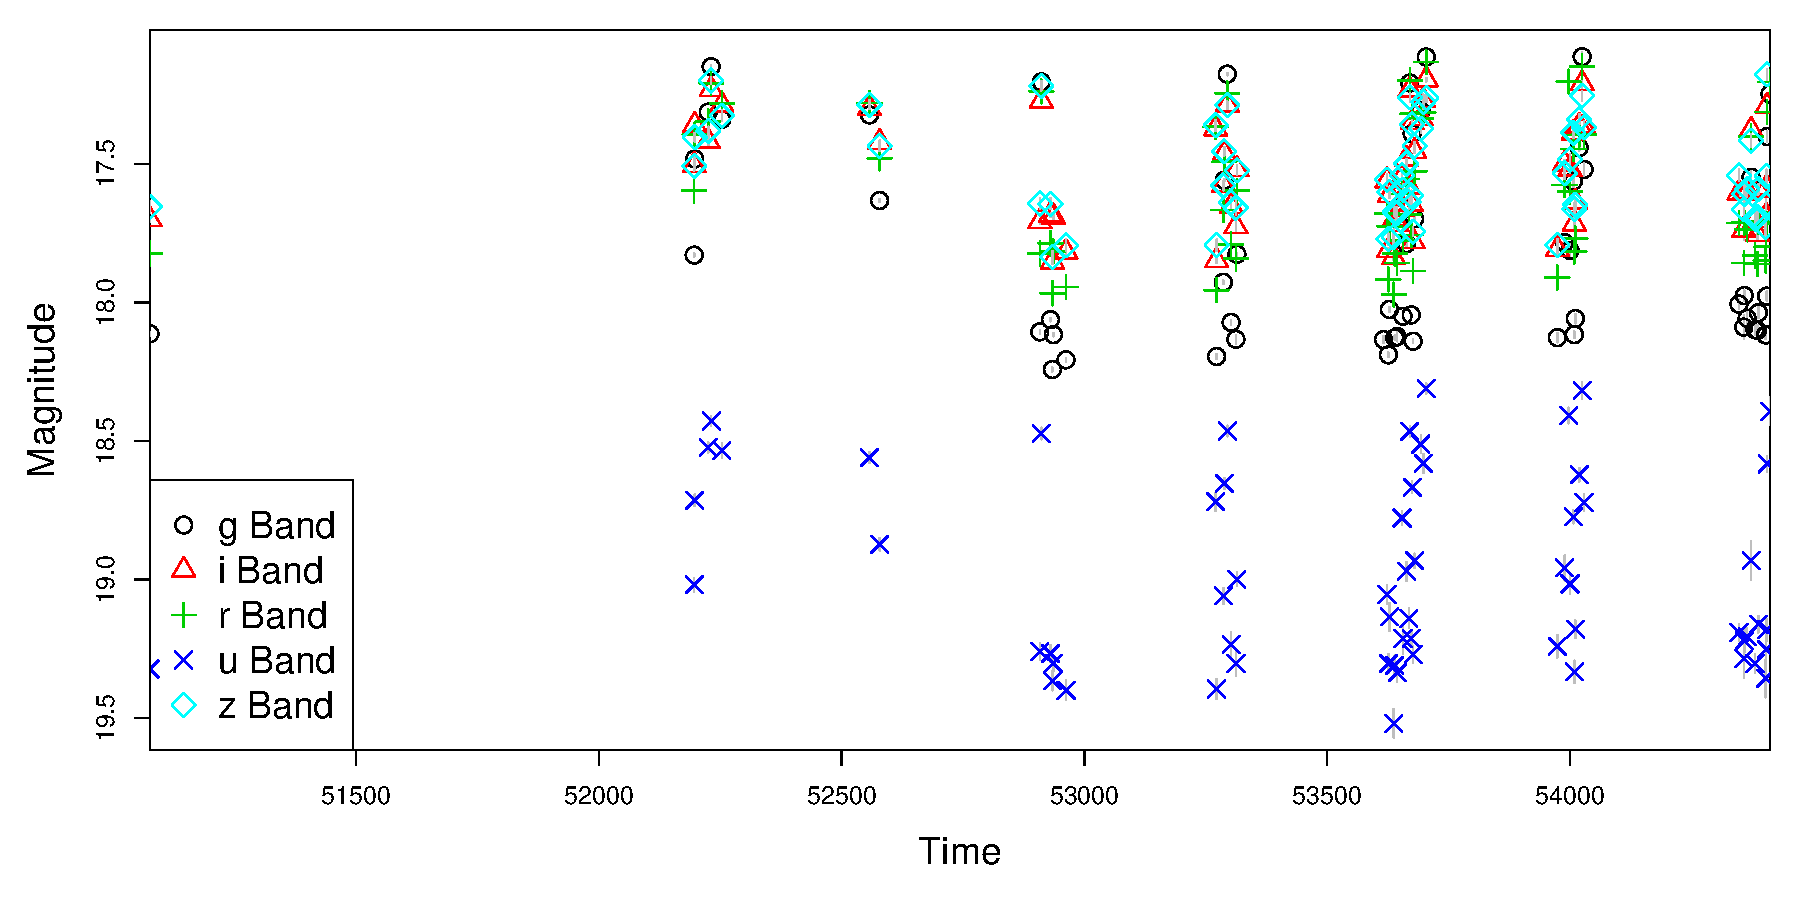
\includegraphics[scale=.15]{figs/unfolded_13350.pdf}
\end{textblock*}


  \begin{textblock*}{3cm}(5.5cm,3.5cm) % {block width} (coords)
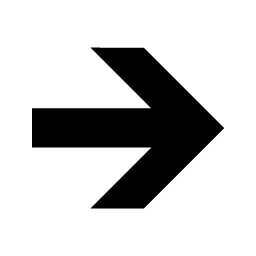
\includegraphics[scale=.15]{figs/rightarrow.png}
\end{textblock*}

  \begin{textblock*}{3cm}(6.75cm,3.1cm) % {block width} (coords)
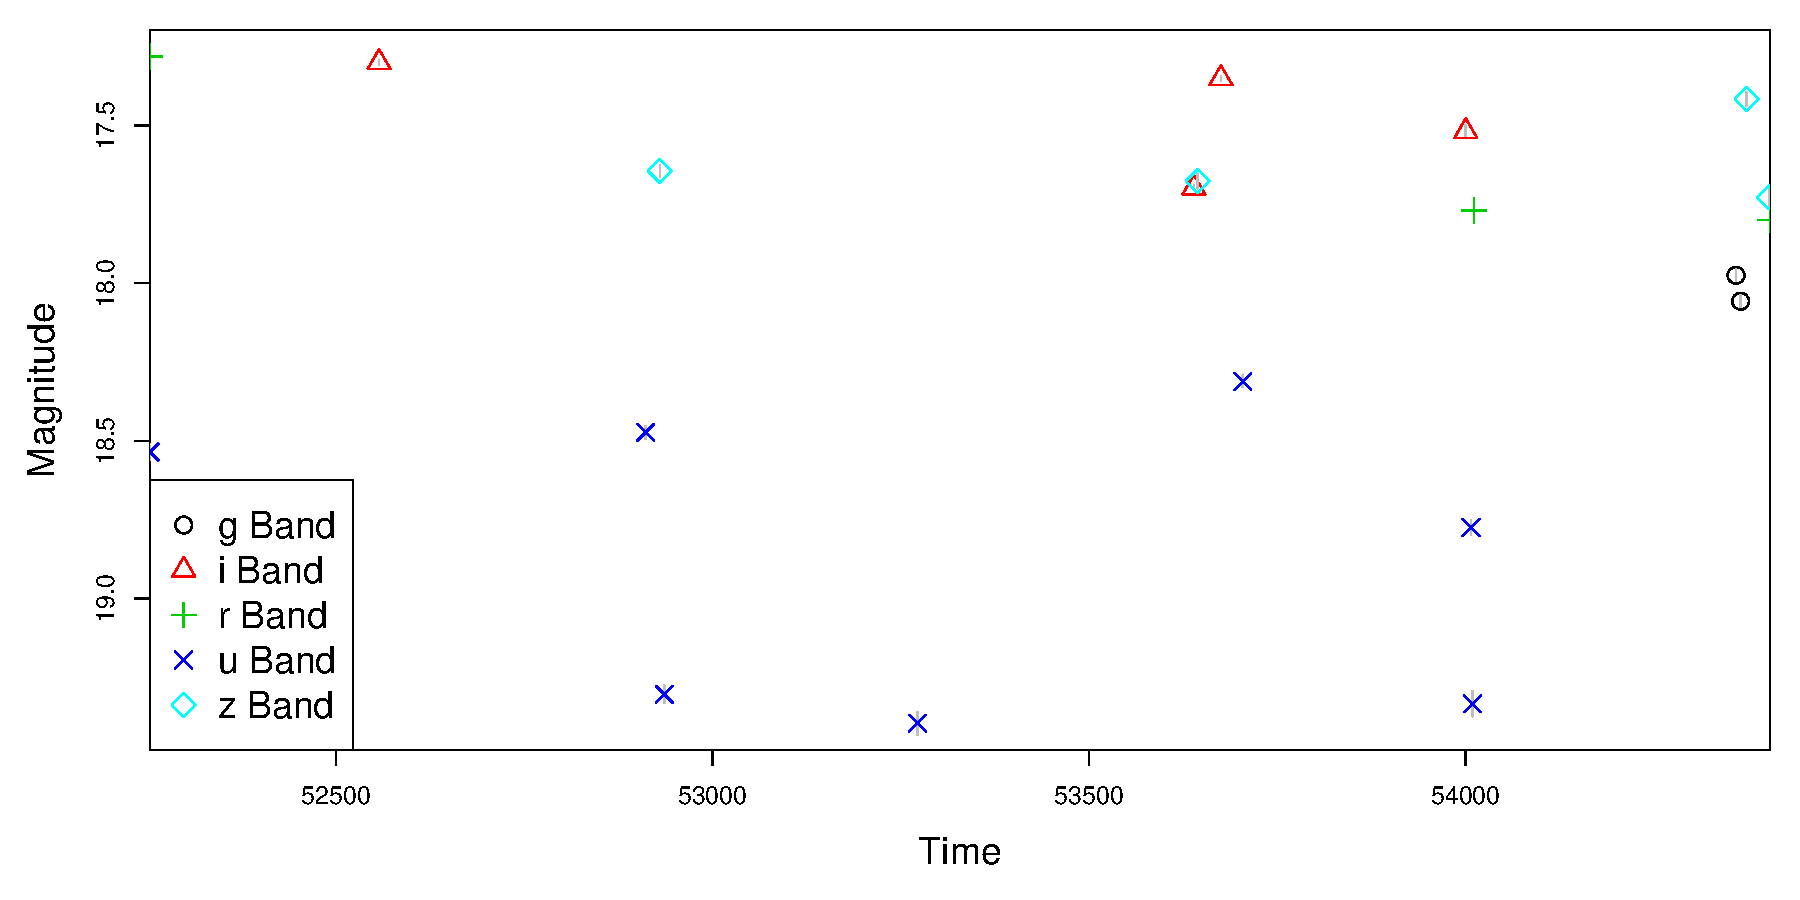
\includegraphics[scale=.15]{figs/unfolded_13350down.pdf}
\end{textblock*}

  \begin{textblock*}{12cm}(1.75cm,6.1cm) % {block width} (coords)
\begin{itemize}
\item Can we estimate periods correctly for RR Lyrae?
\item Can we separate RR Lyrae from non--RR Lyrae? 
\item Can we estimate distances accurately?
\item Can we reproduce halo maps of Sesar 2010?
\end{itemize}
\end{textblock*}

\end{frame}


\begin{frame}{Simulation Results for Period Estimation}



\begin{center}
Comparison of period estimates for 350 RR Lyrae\\
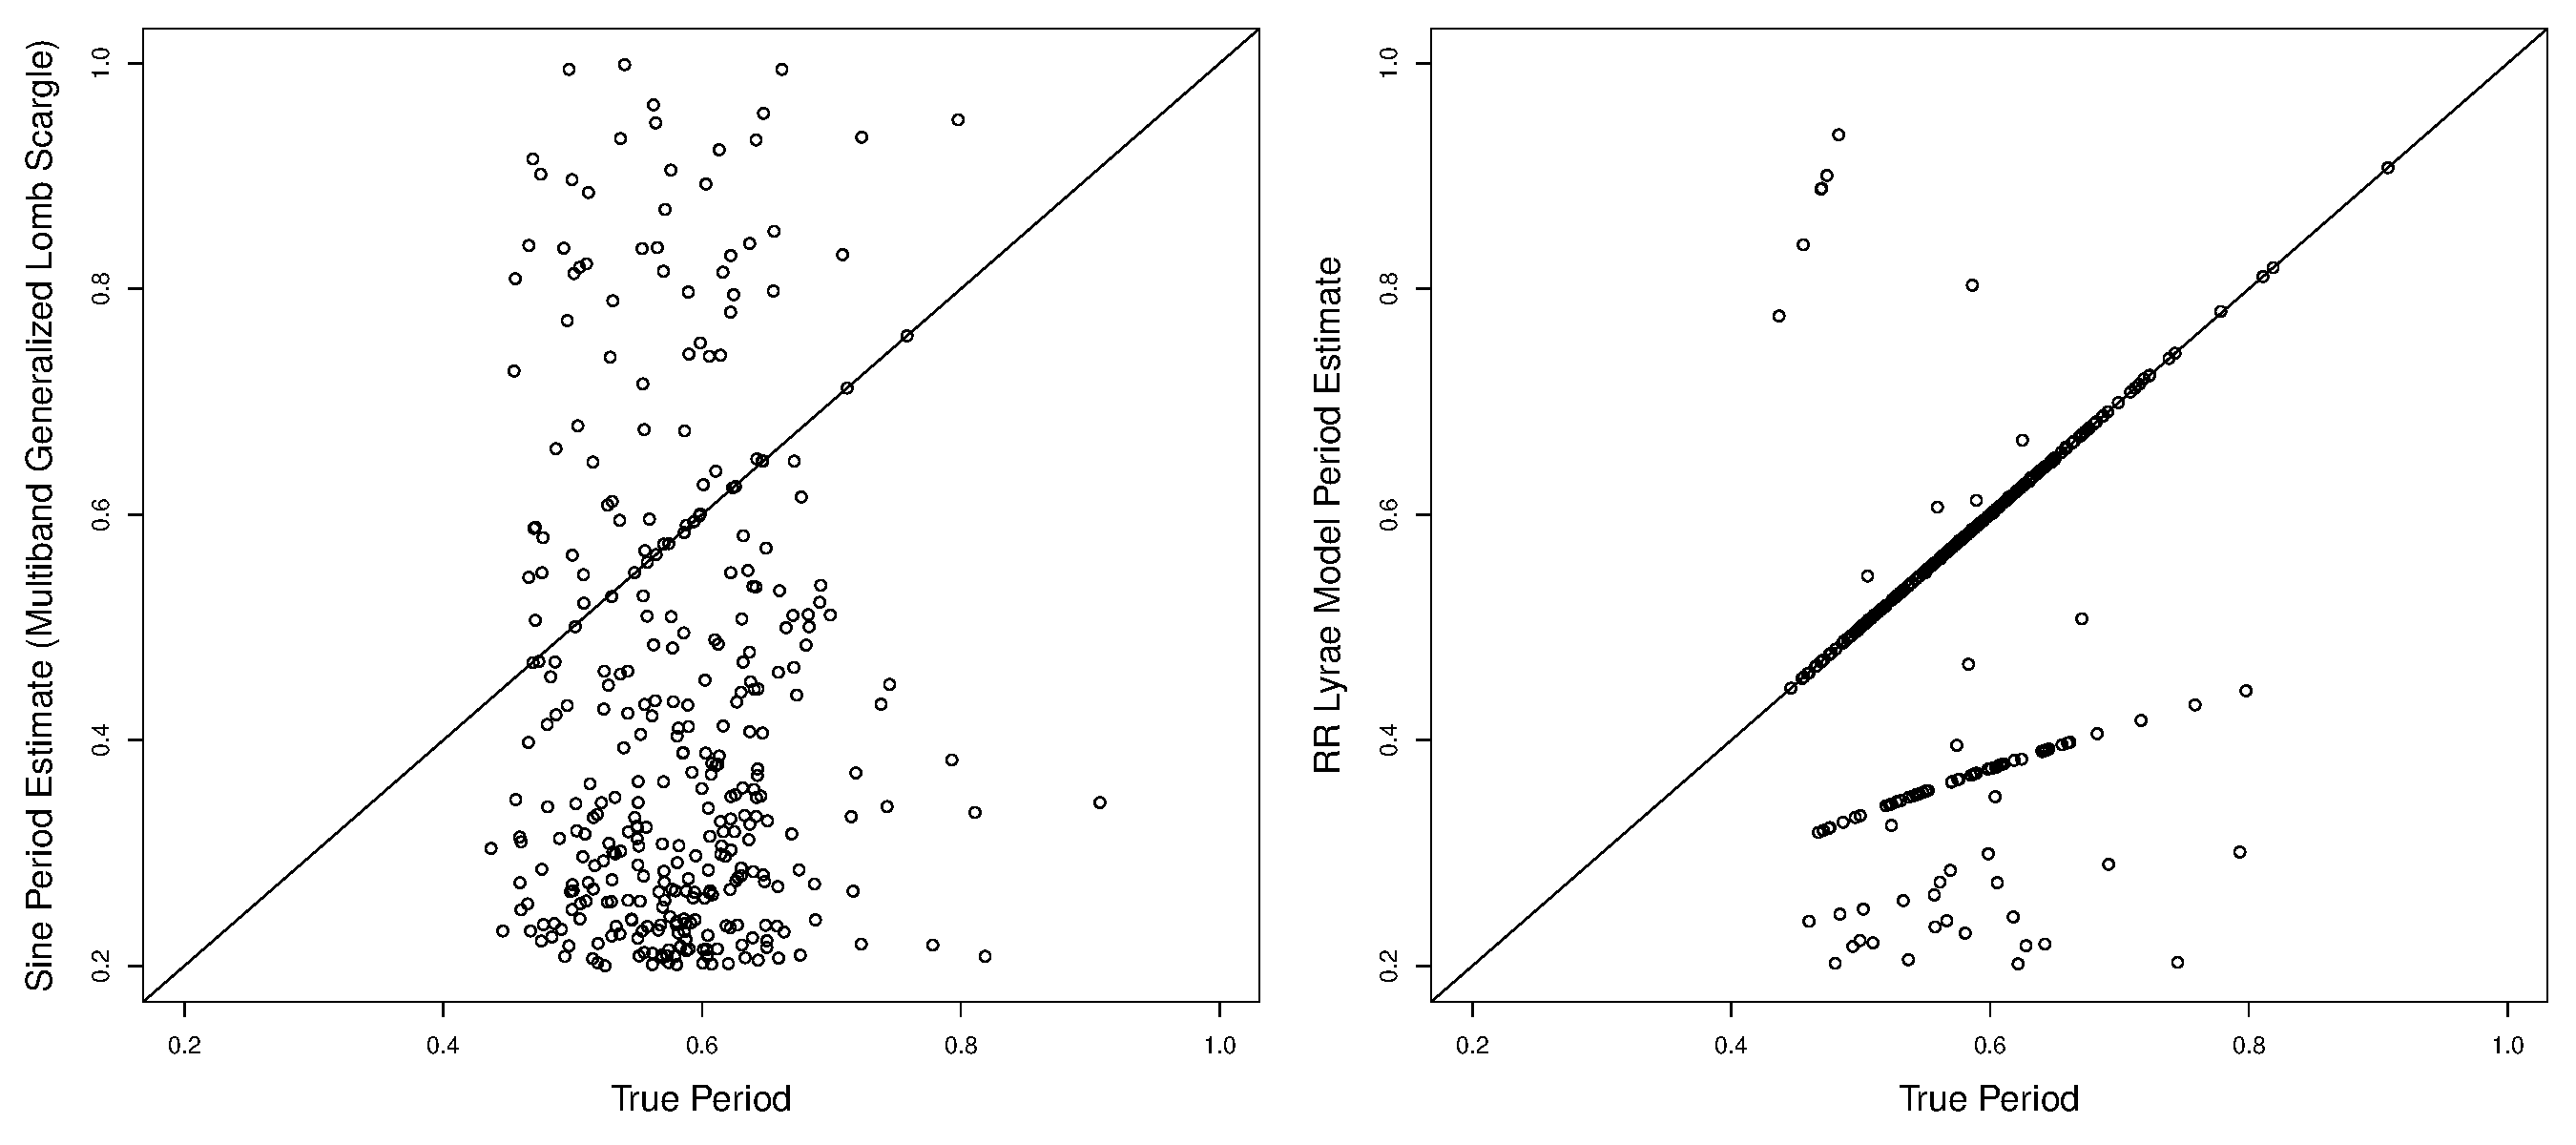
\includegraphics[scale=.25]{figs/period_comparison.pdf}
\end{center}


%% \begin{itemize}
%% \item Sine Model: $6$\% of estimates within $0.01$\% of truth.
%% \item RR Lyrae Model: $67$\% of estimates within $0.01$\% of truth.
%% \end{itemize}

\end{frame}


\begin{frame}{Simulation Results for Classification}

\begin{center}
Downsampled 1000 Not--RR Lyrae and 350 RR Lyrae
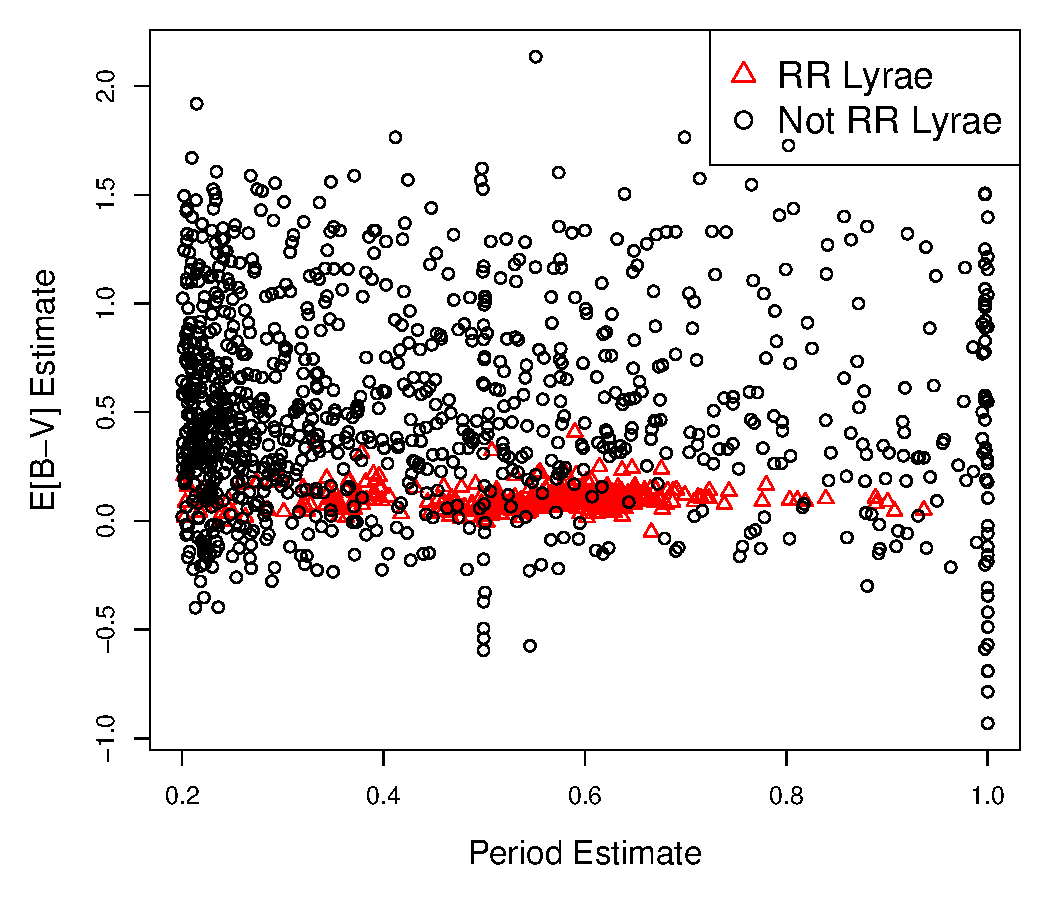
\includegraphics[scale=.33]{figs/period_vs_EBV.pdf}
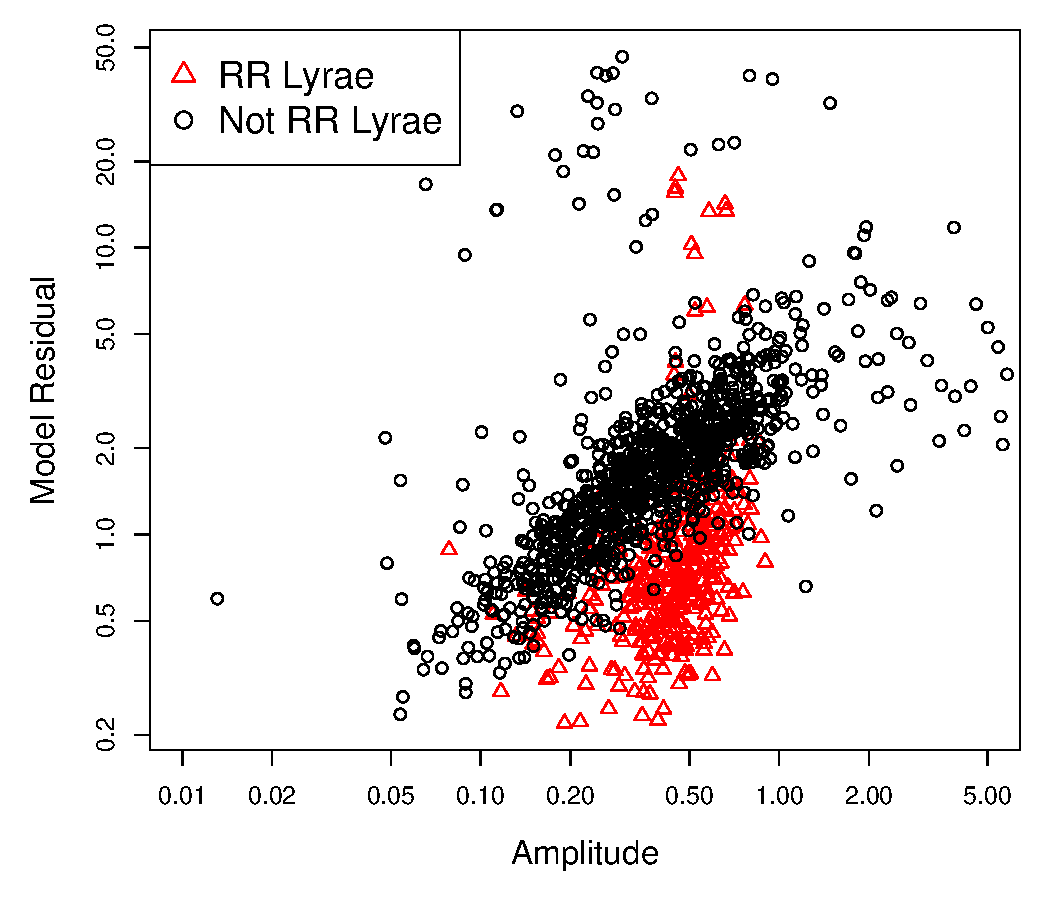
\includegraphics[scale=.33]{figs/a_vs_dev_log.pdf}
\end{center}

\begin{itemize}
\item Visually good separation with small number of features.
\item Potential to use model output as feature input to classifier.
%\item Hernitschek \cite{hernitschek2016finding} used structure functions to classify sparsely sampled RR Lyrae in Pan--STARRS.
\end{itemize}
\end{frame}


\begin{frame}{Simulation Results for Distance Estimation}
\begin{itemize}
\item Use model to estimate distance modulus ($\mu$) for RR Lyrae.
\item Convert $\mu$ to distance (d) in parsecs: $d = 10^{\mu/5 + 1}$
\end{itemize}

\begin{center}
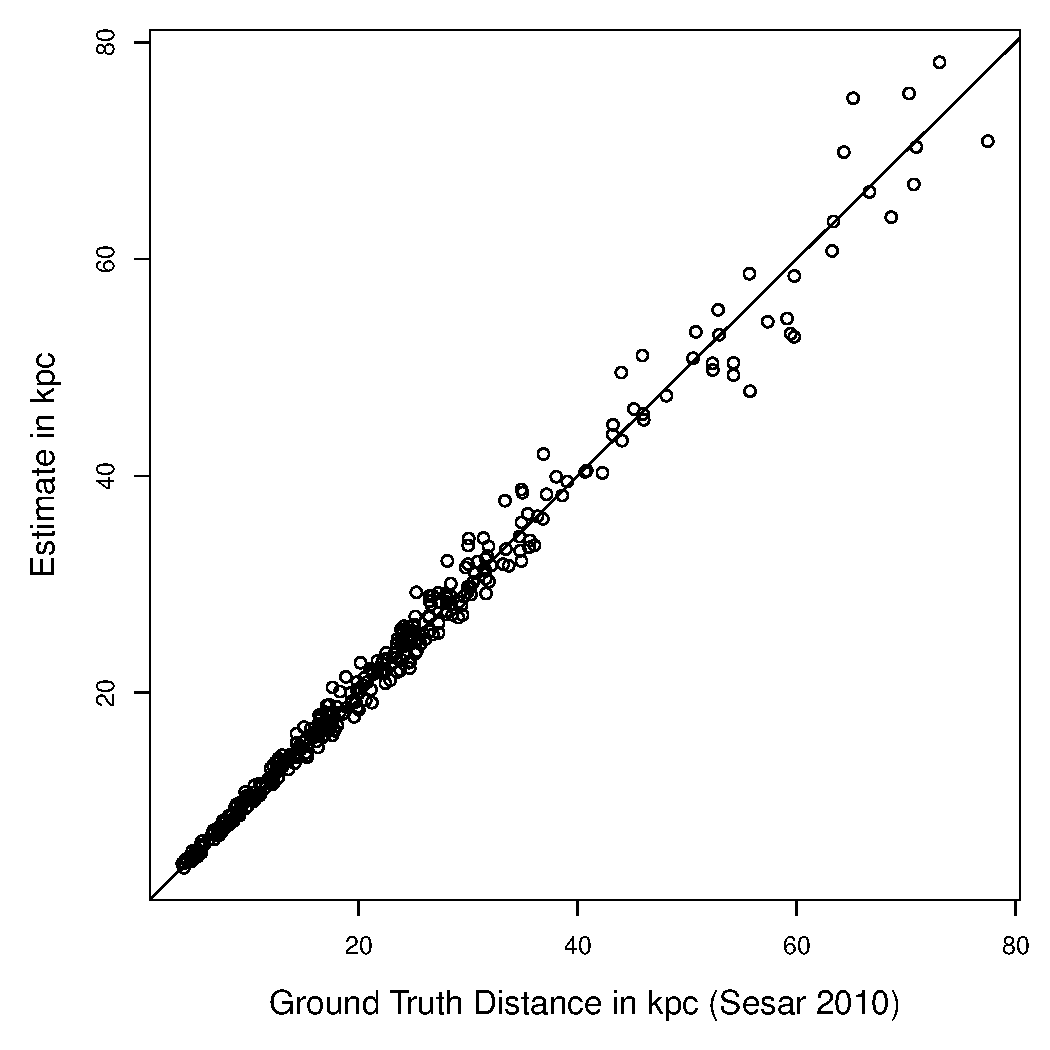
\includegraphics[scale=.35]{figs/distance_comparison.pdf}
\end{center}



\end{frame}


\section{Related and Ongoing Work}

\begin{frame}{Related Work}

\textbf{Period Estimation Algorithms / Variable Star Models:}
\begin{itemize}
\item Sinusoid Based Methods
\begin{itemize}
\item Lomb Scargle (LS) \cite{lomb1976least,scargle1982studies}
\item Generalized LS (GLS) \cite{zechmeister2009generalised}
\item Multiband Extensions \cite{vanderplas2015periodograms,long2014estimating}.
\item AoV \cite{schwarzenberg1996fast}
\end{itemize}
\item ``Non--parametric'' methods
\begin{itemize}
\item Phase Dispersion Minimization \cite{stellingwerf1978period}
\item Supersmoother \cite{sesar2010light}
\end{itemize}
\item Template Based Methods
\begin{itemize}
\item RR Lyrae templates by Sesar \cite{sesar2010light}, Kovacs \cite{kovacs2007computation}
\item Cepheid templates by Pejcha \cite{pejcha2012global}, Yoachim \cite{yoachim2009panoply}
\end{itemize}
\end{itemize}

\vspace{.1in}

\textbf{Finding RR Lyrae in Sparsely Sampled Light Curves:}
\begin{itemize}
\item Hernitschek \cite{hernitschek2016finding} uses structure functions to find RRL / QSO.
\end{itemize}


\end{frame}

\begin{frame}{Ongoing Work}
\begin{itemize}
\item Model refinements:
\begin{itemize}
\item $M_b$ dependence on period, metallicity.
\item Bands other than $g,i,u,r,z$
\item Parameterize $\gamma_b$ to account for shape differences across RRL
\end{itemize}
\item Propagate uncertainty to 3D halo density estimate
\begin{itemize}
\item Treat as Inference Problem: Bayesian posterior or frequentist confidence bands. Hierarchical model?
\item Treat as Prediction Problem: Evaluate distance / density estimates using Stripe 82 data or follow--up observations.
\end{itemize}
\item Milky Way Halo maps using DES data
\end{itemize}
\end{frame}







\begin{frame}{Talking to Statisticians}

\end{frame}


%% \begin{frame}{Conclusions}
%% \begin{itemize}
%% \item Models for specific variable star classes:
%% \begin{itemize}
%% \item Pros: better parameter estimates, improved classification
%% \item Cons: difficult to build, more computation time
%% \end{itemize}
%% \item 
%% \item Survey cadence selection
%% \end{itemize}
%% \end{frame}


\begin{frame}[allowframebreaks]{Bibliography}
%  \def\newblock{\hskip .11em plus .33em minus .07em}
%  \nocite{*}
%\nocite{*}
\bibliographystyle{plain} 
  \tiny{
  \bibliography{refs}}
\end{frame}

\end{document}


